\pdfoutput=1
\documentclass[11pt]{amsart}
\usepackage{amsmath,amssymb,amsthm}
\setcounter{MaxMatrixCols}{11}
\usepackage[margin=1.2in]{geometry}
\usepackage{booktabs,adjustbox,graphicx,xcolor}
\usepackage{tikz}
\usetikzlibrary{arrows.meta,positioning,calc}
\usepackage[colorlinks=true,linkcolor=blue,citecolor=blue,urlcolor=blue]{hyperref}
\hypersetup{pdfauthor={Bernd Johannes Wuebben},pdftitle={Integral topology and small eigenvalues in Calabi-Yau conifold transitions}}
\setlength{\emergencystretch}{2em}
\newtheorem{theorem}{Theorem}[section]
\newtheorem{proposition}[theorem]{Proposition}
\newtheorem{lemma}[theorem]{Lemma}
\newtheorem{corollary}[theorem]{Corollary}
\theoremstyle{definition}
\newtheorem{definition}[theorem]{Definition}
\newtheorem{example}[theorem]{Example}
\theoremstyle{remark}
\newtheorem{remark}[theorem]{Remark}
\newcommand{\ZZ}{\mathbb Z}
\newcommand{\QQ}{\mathbb Q}
\newcommand{\RR}{\mathbb R}
\newcommand{\CC}{\mathbb C}
\newcommand{\PP}{\mathbb P}
\newcommand{\OO}{\mathcal O}
\newcommand{\HH}{\mathcal H}
\newcommand{\ddc}{dd^c}
\newcommand{\vol}{\operatorname{Vol}}
\newcommand{\Ric}{\operatorname{Ric}}
\newcommand{\Rm}{\operatorname{Rm}}
\newcommand{\PD}{\operatorname{PD}}
\newcommand{\Capacity}{\operatorname{Cap}}
\newcommand{\im}{\operatorname{im}}
\newcommand{\coker}{\operatorname{coker}}
\newcommand{\End}{\operatorname{End}}
\newcommand{\reg}{\mathrm{reg}}
\title[Topology and small eigenvalues in conifold transitions]{Integral topology and small eigenvalues\\in Calabi--Yau conifold transitions}
\author{Bernd Johannes Wuebben}
\subjclass[2020]{58J50 (primary); 32Q25, 14J32, 58J05 (secondary)}
\keywords{Calabi--Yau threefold, conifold transition, Hodge Laplacian,
small eigenvalue, integral cohomology, Ricci-flat metric, vanishing cycle}
\date{November 9, 2026\\This version: November 9, 2026}

\begin{document}
\begin{abstract}
We determine the leading small spectrum of the Hodge Laplacian on real
two-forms for Ricci-flat metrics in polarized Calabi--Yau conifold
transitions. We assume a simply connected projective small resolution
and a fixed smoothing that smooths every node to first order, approached
along a fixed ray. Exactly
as many positive eigenvalues tend to zero as there are divisor directions
lost under smoothing, and their decay is inverse-logarithmic in the
smoothing parameter. The leading coefficients are $2\pi$ times the
generalized eigenvalues of the squared exceptional-period form relative
to the harmonic norm after projection off all surviving cohomology.
We compute this norm from global intersections. The divisor-period
restriction map also determines the integral relations among
cohomological vanishing cycles. The small eigenspaces are coexact and
primitive of real type $(1,1)$, with a uniform gap in the remaining
positive two-form spectrum. Applications to four-node and eight-node
toric transitions give three and two distinct coefficients, respectively.
For the sixteen-node split quintic with K\"ahler class
$c_1(\mathcal O(1))$, the coefficient is $10\pi$; we also
calculate its integral rings, attachment and specialization maps,
primitive vanishing lattice and monodromy image of index sixteen.
The resolution and smoothing branches converge to a common Ricci-flat metric
completion, and their tangent Hermitian--Einstein connections converge
smoothly to the central tangent connection on compact subsets of the
regular locus.
\end{abstract}
\maketitle
\section{Introduction}\label{sec:introduction}

We determine the leading small positive two-form eigenvalues of the
Ricci-flat metrics in a polarized Calabi--Yau conifold transition.
Their number is the loss of second cohomology under smoothing. Their
coefficients depend on the periods of divisor classes over exceptional
curves and on the global polarized intersection form. The same period
map determines the integral relations among the vanishing cycles.
Thus the topological and spectral conclusions use the same marked
geometric transition. Local node types alone do not determine either
the compact cohomology ring or these spectral coefficients.

We calculate the global data for the split quintic and for two toric
transitions constructed in earlier work. The two toric applications
use established geometry from the stability--degeneration series and
from the separate Calabi--Yau smoothing series. We denote Papers
IV--VI of the latter series by CY~IV--VI below; these are distinct
from the numbered stability--degeneration papers. The spectral theorem
and its proof come first, followed by the compact applications and the
precise roles of their geometric sources.

\subsection{Geometric hypotheses and the main theorem}
Let $X_0$ be a normal projective threefold with trivial dualizing sheaf,
with exactly $k\geq1$ ordinary double points and no other singularities.
Let
\[
 q:Y\longrightarrow X_0,\qquad
 f:\mathcal X\longrightarrow\Delta
\]
be respectively a projective small crepant resolution and a proper flat
polarized smoothing over a complex disc. Assume that $Y$ is smooth and
simply connected, that the relative canonical bundle of $f$ is trivial,
and that $X_t=f^{-1}(t)$ is smooth for $0<|t|<t_0$. At each node the local
smoothing function $\tau_i$ is required to satisfy
\begin{equation}\label{eq:simple-smoothing}
 \tau_i(0)=0,\qquad \tau_i'(0)\ne0.
\end{equation}
This is a condition on a genuine family over a disc. Let $C_i\simeq\PP^1$
be the exceptional curves and impose
\begin{equation}\label{eq:betti-hypotheses}
 b_2(Y)=2,\qquad b_2(X_t)=1.
\end{equation}
The polarization on $X_0$, its pullback to $Y$, and its extension to $X_t$
are denoted by $H$. It is an integral class, with no implicit factor of
$2\pi$. Choose an integral divisor class $D$ independent of $H$ over
$\RR$, and put
\begin{equation}\label{eq:intersection-data}
 v=H^3,\qquad a=DH^2,\qquad d=D^2H,\qquad
 b_i=D\cdot C_i,\qquad M=\frac{a^2}{v}-d.
\end{equation}
All intersections in this display are taken on $Y$.

On $X_t$ let $g_t$ be the unique Ricci-flat K\"ahler metric with
$[\omega_t]=H$. Let $g_0$ be the singular Ricci-flat K\"ahler metric
in class $H$ on $M_0=X_0^{\reg}$, supplied by \cite{egz,hein-sun}.
By central harmonic representatives we mean smooth $L^2$ two-forms
on $(M_0,g_0)$ that are closed and coclosed. Sections~\ref{sec:mass}
and~\ref{sec:multiple} construct the representatives used below and
justify their domains and uniqueness. We use the nonnegative real Hodge Laplacian
$\Delta_p=dd^*+d^*d$ on real $p$-forms and its ordinary $L^2$ norm.
Write $\lambda_2^+(t)$ for its least strictly positive eigenvalue in
degree two. The subscript indicates form degree. All limits below are
along the fixed positive ray $0<t<t_0$.

\begin{theorem}\label{thm:main}
Under the preceding hypotheses, $M>0$, and
\begin{equation}\label{eq:main-law}
 \lambda_2^+(t)=
 \frac{2\pi\sum_{i=1}^k b_i^2}{M\,|\log t|}(1+o(1)).
\end{equation}
For all sufficiently small $t$, this eigenvalue has real multiplicity one,
and its real eigenspace is generated by a coexact primitive $(1,1)$-form.
There is a constant $\gamma>0$ such that the degree-one spectrum and every
other positive degree-two eigenvalue are at least $\gamma$.
Moreover,
\begin{equation}\label{eq:main-upper}
 \lambda_2^+(t)\le
 \frac{2\pi\sum_i b_i^2}{M\,|\log t|}+C|\log t|^{-2}.
\end{equation}
The constants refer to the fixed family, polarization, ray and local
identifications. No uniformity as the leading coefficients in
\eqref{eq:simple-smoothing} degenerate is asserted.
\end{theorem}

Replacing $D$ by $cD+eH$, with $c\ne0$, multiplies both $M$ and
$\sum b_i^2$ by $c^2$. Thus the coefficient belongs to the one-dimensional
divisor quotient modulo the surviving polarization. It is expressed in
finite global intersection and restriction data; the list of local nodes
alone does not determine it. The theorem gives a matching leading
asymptotic and a sharper one-sided upper estimate. It does not assert a
two-sided second-order remainder.

\subsection{The complete fixed-family cluster}
The same geometric problem allows several divisor directions to be lost.
Retain the preceding family, polarization and simple-smoothing hypotheses,
but replace \eqref{eq:betti-hypotheses} by
$b_2(Y)=b$, $b_2(X_t)=s$ and $m=b-s>0$. Set
\[
 V=H^2(Y;\RR),\qquad r(D)=(D\cdot C_i)_i,\qquad
 K=\ker r,\qquad \mathcal Q=V/K.
\]
The attachment sequence identifies $K$ with the surviving cohomology
$H^2(X_t;\RR)$. Define the forms
\begin{equation}\label{eq:intro-matrix-data}
\begin{split}
 G(D,E)&=-\int_YDEH+
     \frac{3(\int_YDH^2)(\int_YEH^2)}{2\int_YH^3},\\
 \mathcal E([D],[E])&=r(D)\cdot r(E).
\end{split}
\end{equation}
Let $\mathcal M$ be the quotient form induced by $G$ on $\mathcal Q$,
equivalently the minimum squared norm over each coset.
The theorem includes the positivity needed for this definition.
Write $\lambda^+_{2,j}(t)$ for the ordered positive real degree-two
eigenvalues, with multiplicity.

\begin{theorem}\label{thm:matrix}
The form $G$ is the positive-definite inner product of central harmonic
representatives, and $\mathcal E,\mathcal M$ are positive definite on the $m$-dimensional
space $\mathcal Q$. If $0<\mu_1\le\cdots\le\mu_m$ are the
generalized eigenvalues of $\mathcal E$ relative to $\mathcal M$, then
\begin{equation}\label{eq:matrix-law}
 \lambda^+_{2,j}(t)=\frac{2\pi\mu_j}{|\log t|}(1+o(1)),
 \qquad 1\le j\le m.
\end{equation}
The degree-one spectrum and $\lambda^+_{2,m+1}(t)$ have a uniform
positive lower bound. For small $t$, the entire $m$-dimensional positive
small spectral space consists of coexact primitive real $(1,1)$-forms.
A multiplicity-one $\mu_j$ gives an eventually simple eigenvalue.
These assertions concern the fixed family and ray; no uniformity in
degenerating node-scale ratios or two-sided next-order error is asserted.
\end{theorem}

The quotient removes all surviving harmonic directions, rather than
only $H$. It is calculated by the intersection Schur complement
\eqref{eq:mass-schur}. When $b=2$ and $s=1$, this gives the coefficient
of Theorem~\ref{thm:main}; its one-sided sharper upper bound is proved
separately. Section~\ref{sec:multiple} supplies the full kernel
projection and the ordered lower bounds needed for
Theorem~\ref{thm:matrix}.

\subsection{Analytic inputs and proof}
Singular Ricci-flat metric existence, conical regularity and the local
expansions for the actual smoothing metrics are supplied by
\cite{egz,hein-sun,benabida}. They do not determine the compact
small-eigenvalue coefficients. We combine those metric results with
conic spectral compactness and a sharp capacity calculation to prove
\eqref{eq:main-law} and the ordered matrix law \eqref{eq:matrix-law}.

Ann\'e--Takahashi describe the spectral limits in exact-cone surgery
in terms of the central operator, complete-cap harmonic forms and critical
extended solutions \cite{anne-takahashi}. We use their norm decomposition
for finitely many caps, with the critical terms excluded in physical
degrees one and two. The proof then has three steps. The restriction map
fixes the harmonic link periods, and a scalar correction computes the
central harmonic Gram form from intersections. On exactly conical models,
logarithmic cutoffs give upper bounds and cap capacity gives matching lower
bounds on every limiting spectral subspace. Dodziuk's comparison of Hodge
eigenvalues under equivalent metrics transfers the entire ordered cluster
to the actual Ricci-flat family \cite{dodziuk}.

The leading law requires only the $C^0$ condition stated in
Definition~\ref{def:C0-comparison}; its geometric verification is separate
from the model argument. The differentiated estimate of
Proposition~\ref{prop:metric-comparison} is used for the sharper rank-one
upper remainder. Projection off all surviving harmonic classes is performed
on the models, where the needed compact convergence follows from the fixed
central elliptic problem.

\subsection{Three compact applications}
For independent linear forms $l_1,l_2$ and general quartics $q_1,q_2$ on
$\PP^4$, the split quintic $X_0=\{l_1q_2-l_2q_1=0\}$ has sixteen
nodes on the plane $\{l_1=l_2=0\}$. Its incidence resolution lies in
$\PP^4\times\PP^1$, with hyperplane classes $H,L$.

\begin{corollary}\label{cor:quintic}
Let $X_t=\{l_1q_2-l_2q_1+tG=0\}$, where the quintic $G$ is nonzero
at every node. For the Ricci-flat metrics in class $H$,
\[
 \lambda_2^+(t)\sim\frac{10\pi}{|\log t|}.
\]
The eigenvalue has all the simplicity, type, gap and one-sided remainder
properties of Theorem~\ref{thm:main}.
\end{corollary}

Here $r(L)=(1,\ldots,1)$ and $M=16/5$. The same primitive diagonal
vector generates the integral relation among the cohomological vanishing
cycles. The marked transition, including its full integral rings and
monodromy image of index sixteen, is stated in
Theorem~\ref{thm:integrated} and proved in Appendices~\ref{sec:integral-topology}
and~\ref{sec:tangent}.

\subsubsection*{Eight nodes}
Let $B=\PP^1\times\PP^1$ and
$Z=\PP_B(\OO\oplus\OO(1,-1))\times_B
\PP_B(\OO\oplus\OO(1,-1))$. In the quotient convention write
$f,g$ for the base hyperplane classes and $\xi_1,\xi_2$ for the
tautological classes. The anticanonical contraction of a general
anticanonical hypersurface $Y\subset Z$ is the eight-node threefold
$X_0$ constructed in \cite[Appendix~A, Proposition~A.1]{wuebben-chambers}.

\begin{corollary}\label{cor:eight-node}
This transition admits polarized smoothings with trivial relative
canonical bundle and first-order smoothing at every node, whose central
polarization pulls back to
$H=(4g+2\xi_1+2\xi_2)|_Y$. For every such fixed family and ray,
the actual Ricci-flat metrics in class $H$ have precisely two small
positive degree-two eigenvalues, with
\begin{equation}\label{eq:eight-spectral-law}
 \lambda^+_{2,1}(t)\sim\frac{\pi}{|\log t|},\qquad
 \lambda^+_{2,2}(t)\sim\frac{5\pi}{4|\log t|}.
\end{equation}
Both are eventually simple, coexact and primitive real $(1,1)$.
The degree-one spectrum and all other positive degree-two eigenvalues
have a uniform positive lower bound for that fixed family.
\end{corollary}

Here $b_2(Y)=4$ and $b_2(X_t)=2$. The period matrix and the quotient
mass are calculated from the earlier proposition's divisor intersections
and two exceptional-curve types. Section~\ref{sec:eight-node} verifies
the additional polarized-family hypotheses and proves the corollary.
This is an application of Theorem~\ref{thm:matrix}; it makes no new
integral saturation assertion for the eight-node family.

\subsubsection*{Four nodes}
Let $X'_9$ be the four-node partial resolution on the nonmirror side of
\cite[Section~11.1]{wuebben-cy-mirror}, with the chosen projective
small resolution $Y$. Section~\ref{sec:cy-x9} specifies the ample
Cartier class $\mathcal L_0$ by the eleven-ray support vector
\eqref{eq:x9-height}. Write $H=c_1(q^*\mathcal L_0)$.

\begin{corollary}\label{cor:x9}
The threefold $X'_9$ admits a relatively polarized smoothing carrying
exactly $\mathcal L_0$, with trivial relative canonical bundle and
first-order smoothing at every node. One has $b_2(Y)=6$,
$b_2(X_t)=3$ and $H^3=8712$. For every such fixed family and ray,
the actual Ricci-flat metrics in class $H$ have precisely three small
positive degree-two eigenvalues, with
\begin{equation}\label{eq:x9-spectral-law}
\begin{split}
 |\log t|\lambda^+_{2,1}(t)&\longrightarrow\frac{2\pi}{7},\\
 |\log t|\lambda^+_{2,2}(t)&\longrightarrow
       \frac{\pi(375-3\sqrt{3065})}{628},\\
 |\log t|\lambda^+_{2,3}(t)&\longrightarrow
       \frac{\pi(375+3\sqrt{3065})}{628}.
\end{split}
\end{equation}
All three are eventually simple, coexact and primitive real $(1,1)$.
The degree-one spectrum and all other positive degree-two eigenvalues
have a uniform positive lower bound for that fixed family.
\end{corollary}

The source's integral exceptional relation $(1,-1,-1,1)$ supplies a
full-support deformation tangent through
\cite[Theorems~2.5 and~4.5]{wuebben-cy-smoothing}. We prove that the
exact ample class extends, and calculate the full three-dimensional
harmonic quotient. The resulting spectral law is an additional
consequence on the established original-side geometry; it is not a
claim about the mixed-singularity $X_9$ or the distinct mirror family.

\subsection{Relation to earlier work}
The split-quintic construction and conifold attachment sequences are
classical \cite{greene-morrison-strominger,rossi,lee-lin-wang}.
Our two toric applications use specific earlier geometric constructions:
\cite[Appendix~A, Proposition~A.1]{wuebben-chambers} supplies the eight-node
contraction and Picard rank, while \cite[Section~11.1]{wuebben-cy-mirror}
supplies the four-node threefold $X'_9$ and its exceptional circuits.
The nodal specialization of \cite[Theorems~2.5 and~4.5]{wuebben-cy-smoothing}
provides the latter's deformation tangent and smooth deformation base.
In both applications we check first-order smoothing and extension of the
specified ample class before applying the spectral theorem.

The curve-class map and the divisor-period map are transposes:
\begin{equation}\label{eq:curve-period-duality}
 A:\QQ^k\longrightarrow H_2(Y;\QQ),\quad e_i\longmapsto[C_i],
 \qquad r=A^*,\qquad \im r=(\ker A)^\perp.
\end{equation}
The space $\ker A$ governs localized deformation tangents, whereas $\ker r$
is the surviving second cohomology and $\im r$ supplies the spectral
periods. The harmonic quotient also requires the polarized intersection
form. Integral saturation is proved from the actual attachments where it
is asserted; it does not follow from \eqref{eq:curve-period-duality}.

Ann\'e--Takahashi's conic surgery theorem includes logarithmic modes
\cite{anne-takahashi}. Rowlett proves spectral and heat convergence under
her asymptotically conic convergence hypotheses \cite{rowlett}.
Guillarmou--Sher's low-energy resolvent theorem \cite[Theorem~1]{guillarmou-sher}
excludes the harmonic link two-form channel present here through its
condition~(4). For scalar Laplacians in different degenerations, Cao proves
two-sided inverse-logarithmic orders for induced total-space metrics
\cite[Theorems~0.2--0.4]{cao}, and Dai--Yoshikawa obtain small-eigenvalue
orders and the leading product in reduced curve degenerations
\cite[Theorems~0.2--0.3]{dai-yoshikawa}. These results concern different
operators and metrics. Here the conclusion is the individual leading
coefficient of every lost-divisor mode for the actual polarized Ricci-flat
metrics, computed from the full quotient harmonic norm.

The tangent connections in Appendix~\ref{sec:tangent} are induced by those
Ricci-flat metrics. Collins--Picard--Yau treat tangent-bundle HYM geometry
on balanced conifold transitions \cite{collins-picard-yau}; our appendix
identifies the flat tangent-sheaf limit and its reflexive hull for the
specified K\"ahler family.

Section~\ref{sec:geometry} establishes the actual metric comparison.
Section~\ref{sec:mass} calculates the harmonic norm and the integral
restriction map. Sections~\ref{sec:capacity}--\ref{sec:multiple} prove the
model spectral law, transfer it using only $C^0$ comparison, and isolate
the stronger rank-one remainder. Sections~\ref{sec:quintic},
\ref{sec:eight-node} and~\ref{sec:cy-x9} give the three applications.
The appendices retain the supporting integral and tangent calculations.

\section{Conifold geometry and actual metric comparison}\label{sec:geometry}

\subsection{The link and its integral normalization}
An ordinary double point is analytically the cone $\sum_{j=1}^4z_j^2=0$.
Its Ricci-flat metric cone is $g_C=dr^2+r^2h$, where the homogeneous
metric on $T^{1,1}\simeq S^2\times S^3$ is
\begin{equation}\label{eq:link-metric}
 h=\frac19\eta_c^2+
 \frac16\sum_{j=1}^2(d\theta_j^2+\sin^2\theta_j\,d\phi_j^2),\qquad
 \eta_c=d\psi+\cos\theta_1d\phi_1+\cos\theta_2d\phi_2.
\end{equation}
Here $\psi$ has period $4\pi$ and $\Ric_h=4h$.
Put $\sigma_j=\sin\theta_jd\theta_j\wedge d\phi_j$ and
\begin{equation}\label{eq:link-form}
 \vartheta=\frac{\sigma_1-\sigma_2}{8\pi}.
\end{equation}
The circle bundle over $\PP^1\times\PP^1$ has Chern class $(1,1)$ up
to a common sign. A primitive two-cycle projects with degrees $(1,-1)$;
therefore $\vartheta$ has period one. It is harmonic: it is closed,
its horizontal part is anti-self-dual, and wedging that part with
$d\eta_c=-(\sigma_1+\sigma_2)$ gives zero. In the orthonormal frame,
\begin{equation}\label{eq:link-norm}
 |\vartheta|_h^2=\frac9{8\pi^2},\qquad
 \vol(T^{1,1},h)=\frac{16\pi^3}{27},\qquad
 c:=\|\vartheta\|_{L^2(h)}^2=\frac{2\pi}{3}.
\end{equation}
The selected small-resolution ruling fixes the sign of its primitive
period. On a cone, $\vartheta$ is a primitive real $(1,1)$-form, of
pointwise size $O(r^{-2})$.

The smoothing cap is $T^*S^3$ with the Stenzel metric, asymptotic with
positive differentiated rate to this cone \cite{stenzel,candelas-ossa}.
The small-resolution cap is the total space of
$\OO_{\PP^1}(-1)^{\oplus2}$ with its Ricci-flat resolved-conifold metric.
The two caps have the same link but retain different primitive cohomology:
restriction to the link is an isomorphism in degree three for the smoothing
cap and in degree two for the resolution cap.

\subsection{The central metric and the smoothing scale}
Let $X_0^\reg$ carry the singular Ricci-flat K\"ahler form $\omega$ in
class $H$. The bounded-potential construction \cite[\S7.2, Theorem~7.5 and Corollary~7.6]{egz} gives a closed positive pullback current on $Y$. Its
Bedford--Taylor products have their cohomological masses and give no mass
to the exceptional analytic set. The conical theorem of Hein--Sun
\cite[Theorem~1.4 and Corollary~1.5]{hein-sun} supplies holomorphic node
charts such that, for some $\mu>0$,
\begin{equation}\label{eq:central-rate}
 |\nabla_C^j(g_0-g_C)|_{g_C}\le C_jr^{\mu-j}
 \quad (j\ge0).
\end{equation}
Use the minimum rate over the finitely many ends. Benabida's Theorem~A
provides the corresponding polyhomogeneous expansion \cite{benabida}.
The cited metric theorems use the class $2\pi c_1(\mathcal L)$ for
the polarizing line bundle $\mathcal L$. We rescale their metrics by
$(2\pi)^{-1}$ to obtain our class $H=c_1(\mathcal L)$, with the corresponding fixed rescaling
of cone radii and cap normalizations. Written as $dr^2+r^2h$, the
normalized link metric and \eqref{eq:link-norm} are unchanged.

Condition~\eqref{eq:simple-smoothing} makes the total-space projection a
holomorphic Morse function near each node. The local family therefore
has the weighted ordinary-node model, with weights $3/2$ on the coordinates
and $3$ on the algebraic smoothing parameter. This model is compatible
with the central conical chart. Indeed, the transition between two
ordinary-quadric charts lifts to an ambient holomorphic germ $\Phi$ with
$Q\circ\Phi=uQ$, where $Q=\sum z_j^2$ and $u$ is a holomorphic unit.
Its linear part $A$ satisfies $Q(Az)=u(0)Q(z)$ and extends to the
weighted smoothing after a fixed rescaling of the base. Since all
coordinate weights are $3/2$, the terms $\Phi-A=O(|z|^2)$ have relative
conic order $O(r^{3/2})$, with differentiated bounds. After this linear
normalization, \eqref{eq:central-rate} therefore holds in the family
chart, with $\mu$ decreased if necessary. Along the fixed positive ray
we use the reference metric scale
\begin{equation}\label{eq:metric-scale}
 \epsilon=t^{1/3}.
\end{equation}
On the smoothing branch, metrics, K\"ahler forms and eigenvalues indexed
by $\epsilon$ are evaluated at the algebraic parameter $t=\epsilon^3$.
The individual cap scales have fixed positive leading ratios to $\epsilon$.
Multiplying a local normalization by a fixed constant changes a logarithmic
length by a bounded term.

\begin{lemma}[Uniform corner extraction]\label{lem:corner-extraction}
Let $f(\rho_1,\rho_2,y)$ be a polyhomogeneous tensor coefficient on a
compact product corner. Suppose its index sets at both faces have only
log-free order-zero terms and terms of strictly positive real order, and
let $f_0(\rho_1,y)$ be its trace at $\rho_2=0$. There is $a_0>0$ such
that, for every fixed number of b-derivatives,
\begin{equation}\label{eq:corner-extraction}
 |D_b^j(f-f_0)|\le C_j\rho_2^{a_0}
\end{equation}
uniformly up to $\rho_1=0$.
\end{lemma}
\begin{proof}
Discreteness of the index set gives a positive gap above zero at the
$\rho_2$ face. Choose $a_0$ below that gap and a positive remainder order.
Expansion coefficients and their fixed b-derivatives are bounded at the
other face, since its index set has no negative orders or order-zero
logarithms. Subtracting the trace removes the order-zero term; positive
powers absorb the remaining finite logarithmic powers. The conormal
remainder has the same bound. A finite corner cover makes the constants
uniform. Pointwise convergence at fixed $\rho_1>0$ alone would not imply
this conclusion.
\end{proof}

\begin{proposition}[Actual metric comparison]\label{prop:metric-comparison}
There are collar-compatible exterior identifications $F_\epsilon$ and
constants $a_0>0$, $r_0>0$ such that, for fixed sufficiently large $A$,
\begin{equation}\label{eq:actual-comparison}
 |\nabla_C^j(F_\epsilon^*g_\epsilon-g_0)|_{g_C}
 \le C_j(\epsilon/r)^{a_0}r^{-j},
 \quad A\epsilon\le r\le r_0,\quad j=0,1.
\end{equation}
The same comparison holds for the K\"ahler forms. On fixed exterior
compact sets the $C^1$ differences are $O(\epsilon^{a_0})$.
On fixed compact subsets of each rescaled cap, the metrics converge in
all derivatives to the normalized Stenzel metric.
\end{proposition}

\begin{proof}
We use the construction of \cite[Theorem~C]{benabida}, with the following
finite-node extension and tensor deduction. The cited work is published;
our numbered references to its proof refer to arXiv version~3, as specified
in the bibliography. Remark~5.2 there describes the extension, but its
Lemma~5.4 is formulated with one cap face. We give the global estimate
needed to replace that hypothesis.

\emph{The normalized scalar inverse.}
Let $\rho_\epsilon$ be a positive radius, equal to the central radius on
the necks and comparable to $\epsilon$ on the cores. For $-4<\beta<0$ put
\[
 \|u\|_{H_\beta^q}^2=
 \sum_{j=0}^q\int |\rho_\epsilon^{j-\beta}\nabla^ju|^2
                         \rho_\epsilon^{-6}\,dV.
\]
The CS space in \cite[Definitions~11.1 and~11.6]{pacini} is the connected
central regular locus; the AC space is the disjoint union of the normalized
Stenzel caps. Disconnected AC spaces are allowed. All ends are filled at
scale $\epsilon$, with fixed ratios absorbed into the caps. Choose a smooth
density $\zeta$ of integral one supported in a fixed central compact set.
Theorem~12.3(1) of \cite{pacini} gives the estimate
\begin{equation}\label{eq:uniform-scalar-inverse}
 \|u\|_{H_\beta^{q+2}}\le C_q\|\Delta_\epsilon u\|_{H_{\beta-2}^q},
 \qquad u\in E_\epsilon:=\left\{\int\zeta u=0\right\},
\end{equation}
uniformly in $\epsilon$, for its parametric connected-sum metric. The
complement is precisely the pullback of the fixed central complement in
that proof: the cutoff used there is one on $\operatorname{supp}\zeta$.
The restricted Laplacian has the same image as the full Laplacian. On the
connected closed smoothing this image is
$\{f:\int f\,dV_\epsilon=0\}$, and the kernel is the single space of
constants. Thus the range condition is global; there is no separate
normalization or mean-zero condition for each cap.

The initial K\"ahler tensor in \cite[Proposition~5.9]{benabida} has the
prescribed central and cap traces with positive orders at the opposite
faces. Compare it with Pacini's metric, interpolated at
$r=\epsilon^\tau$, $0<\tau<1$. On the central and cap sides, its initial
face expansions give errors bounded by positive powers of
$\epsilon^{1-\tau}$ and $\epsilon^\tau$. On the intervening annuli,
\eqref{eq:central-rate} and the AC rate give the same conclusion in every
fixed scaled differentiability norm. Therefore
\[
 \|\Delta_{\rm initial}-\Delta_{\rm Pacini}\|
       _{H_\beta^{q+2}\to H_{\beta-2}^q}=o(1).
\]
Absorption in \eqref{eq:uniform-scalar-inverse} proves the estimate for the
initial family and its subsequent boundary-vanishing formal corrections.
This comparison uses the initial compactification, not any estimate for
the final Ricci-flat metric. Theorem~11.7 of \cite{pacini} supplies the
uniform scaled Sobolev and multiplication estimates used in the nonlinear
argument.

\emph{Finite-node formal corrections.}
The surgery space has one connected central face and finitely many pairwise
disjoint cap faces. The central coefficient problems of
\cite[\S\S5--6]{benabida} are scalar equations on that one connected
conifold, with one integral compatibility condition. The finite-end
positive-weight inverse includes the low harmonic terms at every end
\cite[Proposition~3.4]{benabida}. These terms cannot be discarded when
differentiating the potentials. For the node, the first scalar link
eigenvalues are $0,33/4,12$, with growth rates $0,3/2,2$; below growth two
the terms are constants and the real and imaginary parts of the four
holomorphic linear coordinates \cite[Theorem~2.14(1), Example~2.16]{hein-sun}.
Extend the corresponding central holomorphic germs through the smoothing
charts and multiply by disjoint cutoffs equal to one near the nodes.
Their fibrewise $\partial\bar\partial$ vanishes near the corners, and
all cutoff derivatives have fixed exterior support. Consequently the low
terms introduce no negative corner tensor order.

The AC coefficient equations are a finite direct sum of the inverses in
\cite[Proposition~3.6]{benabida}. Their decaying weight range has no
componentwise integral obstruction. The global volume normalization gives
the compatibility for the central equation. More explicitly, each cap's
volume starts at order $\epsilon^6$, so a central residual coefficient
of order less than six has zero integral by the push-forward argument of
\cite[Proposition~5.5]{benabida}. At the next stage one improves the
central residual to almost order six and the cap residuals to almost order
four, factors out $\epsilon^{4-\eta}$ for a sufficiently small $\eta>0$,
and repeats the same procedure. Multiplication by this scalar preserves
the global zero-integral identity. Cap contributions add in that identity;
they are not required to vanish individually. Finitely many disjoint faces
permit common choices of weights and the same Borel summation.

At a product corner write $\epsilon=\rho_1\rho_2$. The tensor orders in
\cite[proof of Proposition~6.1]{benabida} are the following. A central
potential correction $\epsilon^\delta w$, after removing the
pluriharmonic terms just treated, has $w$ of weight $a>2-\delta$.
Choose $\max(\delta/2,2-a)<\delta'<\delta$. Its twice-differentiated
conic tensor has order
\[
 \rho_2^{\delta'}\rho_1^{a-2+\delta'}.
\]
Both exponents are positive, logarithms are absorbed by the loss in
$\delta'$, and $2\delta'>\delta$ improves the nonlinear residual.
A cap correction has tensor order
$\rho_1^{\delta'}\rho_2^{a+2+\delta'}$, with positive exponents;
the cap weight choice preserves the previously improved central order.
These are tensor estimates, not merely positive orders for potentials.

The inverse \eqref{eq:uniform-scalar-inverse} and the scaled nonlinear
bounds give the final correction as in \cite[\S7]{benabida}. With the
same normalization for every order, uniqueness and Sobolev embedding give
\[
 |\nabla^j\phi_\epsilon|\le C_{N,j}\epsilon^N
                           \rho_\epsilon^{\beta-j}
 \quad\text{for every fixed }N,j.
\]
Since $\epsilon=\rho_1\rho_2$ and $\rho_\epsilon$ is comparable to
$\rho_1$, its metric correction is flat at both faces after any fixed
number of conic derivatives. Joint flatness follows by differentiating
the normalized parameter equation: the coefficient derivatives cost only
fixed powers, and the same uniform linearized inverse gives the displayed
arbitrary-order decay inductively. Thus fibrewise estimates are not being
used alone to infer transverse regularity.

The final tensors consequently have nonnegative polyhomogeneous index
families in the vertical conic bundles: the order-zero term at each face
is log-free, and every other exponent has positive real part. The face
values asserted in Theorem~C are unchanged. The central value is the full
$g_0$; on a cap, $\epsilon^{-2}g_\epsilon$ restricts to its normalized
Stenzel metric. In the conic bundle the latter is
$\rho_2^2g_{\rm St}$ in the cap b-frame. Since
$\rho_2=(1+\widetilde r^2)^{-1/2}$, it is bounded up to the corner
and has the cone trace there.

\emph{Extraction in the conic frame.}
The index families just obtained satisfy Lemma~\ref{lem:corner-extraction}.
Map $(y,r,0)$ to $(y,r,\epsilon/r)$, taking $r=\rho_1$. The vertical
b-frame is $\rho_1\partial_{\rho_1}-\rho_2\partial_{\rho_2},\partial_y$.
After division by $\rho_1$ its pullback is the cone frame
$\partial_r,r^{-1}\partial_y$. A cone covariant derivative costs $r^{-1}$
and bounded b-differentiation. Equation~\eqref{eq:corner-extraction} gives
\eqref{eq:actual-comparison}. Extend the prescribed collar lifts by a
partition of unity on the smooth fixed exterior; their flow gives compatible
identifications. There is no holomorphicity requirement. The exterior and
rescaled-cap estimates follow from the respective face restrictions. The
same argument applies to the K\"ahler tensors.

Finally, the initial form in \cite[Proposition~5.9]{benabida} is obtained
from curvature on the actual polarizing line bundle. The Stenzel form has
a global potential, and the gluing and all subsequent corrections are
fibrewise $\partial\bar\partial$-exact. The construction therefore stays
in $2\pi c_1(\mathcal L_t)$. Ricci-flat uniqueness in this class, followed
by the fixed rescaling already specified, identifies it with $g_t$ on the
prescribed complex family.
\end{proof}

The trace in \eqref{eq:corner-extraction} is the full central tensor.
Comparing both metrics separately with the cone would leave an
$O(r^\mu)$ term independent of $\epsilon$; that weaker estimate is not
used for the differentiated remainder argument.

\section{Harmonic representatives and intersection mass}\label{sec:mass}

\subsection{The two global cohomology directions}
Write $M_0=X_0^\reg=Y\setminus\bigcup_iC_i$. Removing a submanifold of
real codimension four does not change cohomology in degrees one and two.
The Thom sequence consequently gives
\begin{equation}\label{eq:central-cohomology}
 H^1(M_0;\RR)=0,\qquad H^2(M_0;\RR)=\RR H\oplus\RR D.
\end{equation}
The common exterior has boundary a disjoint union of copies of
$S^2\times S^3$. In the smoothing each filling has zero second
cohomology. Mayer--Vietoris therefore identifies the image of $H^2(X_t)$
in $H^2(M_0)$ with the kernel of restriction to these links. This image
is exactly $\RR H$, and the restriction vector of $D$ is $(b_i)$.
In particular it is nonzero. In fact $b_i\ne0$ for every $i$: otherwise
$H\cdot C_i=D\cdot C_i=0$ would make the effective curve $C_i$
numerically zero against every divisor class on the projective $Y$.

The smooth fibres are simply connected. This follows from van Kampen,
since replacing either filling by the other preserves the fundamental
group: the fillings and links are simply connected. Both $Y$ and $X_t$ are compact, simply
connected K\"ahler threefolds with trivial canonical bundle, and admit
Ricci-flat metrics. They have full $\mathrm{SU}(3)$ holonomy in this setting. A nontrivial de Rham decomposition would have
a one-complex-dimensional Ricci-flat factor, whose compact simply
connected cover cannot exist; the irreducible hyperk\"ahler alternative
has even complex dimension. Thus $H^{2,0}(Y)=0$, consistently with the
divisor interpretation of all real second-cohomology directions.

\begin{proposition}\label{prop:mass}
There is a real closed $(1,1)$-form $\eta$ on $M_0$ representing $D$,
with $\Lambda_\omega\eta=3a/v$, such that
\begin{equation}\label{eq:primitive-form}
 \alpha=\eta-\frac av\omega
\end{equation}
is closed, coclosed, primitive and in the Friedrichs form domain.
For some $\nu>0$ its expansion on end $i$ is
\begin{equation}\label{eq:alpha-expansion}
 \alpha=b_i\vartheta_i+O(r^{\nu-2}),\qquad
 \nabla_C^j(\alpha-b_i\vartheta_i)=O(r^{\nu-2-j}),
\end{equation}
for every $j\ge0$. Its norm and orthogonality are
\begin{equation}\label{eq:mass-identity}
 \|\alpha\|_{L^2(g_0)}^2=\frac{a^2}{v}-d=M>0,
 \qquad \langle\alpha,\omega\rangle_{L^2}=0.
\end{equation}
\end{proposition}

\begin{proof}
We use $d^c=\frac i2(\bar\partial-\partial)$, so $dd^c=i\partial\bar\partial$.
Choose a smooth Hermitian metric on the line bundle with class $D$ on
$Y$, and let $\theta_b$ be its real normalized curvature form. A local
small-resolution neighborhood retracts onto its exceptional $\PP^1$.
The node is rational, and the higher direct images of its structure sheaf
vanish. On the inverse image of a sufficiently small Stein neighborhood,
$H^1(\OO)=H^2(\OO)=0$; equivalently one can use the infinitesimal-neighborhood
filtration with quotients $\OO(n)^{\oplus(n+1)}$. The exponential sequence
identifies the local Picard group with $\ZZ$, by exceptional degree.
Thus the line bundle is the $b_i$th power of the selected ruling bundle.

The normalized curvature $\sigma_1/(4\pi)$ of that ruling differs from
\eqref{eq:link-form} by $(\sigma_1+\sigma_2)/(8\pi)$, a constant
multiple of $dd^c\log r$. Changing the local Hermitian metric therefore
makes its curvature $b_i\vartheta_i$. The local logarithmic metric ratios
$u_i$ satisfy $u_i=O(1+|\log r|)$ and
$\nabla_C^ju_i=O(r^{-j})$ for $j\ge1$. Patch them with disjoint cutoffs.
Then
\[
 \theta=\theta_b+dd^cu
\]
is a global real closed $(1,1)$-form representing $D$, equal to
$b_i\vartheta_i$ near each end. The original smooth curvature has
cone size $O(r^{-2})$ with differentiated bounds. Since the cone charts
are holomorphic, type is preserved in this construction. Cone primitivity
and \eqref{eq:central-rate} give
$\Lambda_\omega\theta=O(r^{\mu-2})$.

The bounded-potential intersection products on $Y$ give
\begin{equation}\label{eq:base-intersections}
 \int_{M_0}\omega^3=v,\qquad
 \int_{M_0}\theta_b\omega^2=a,\qquad
 \int_{M_0}\theta_b^2\omega=d.
\end{equation}
For the mixed products, pairing the closed current with smooth closed
forms gives their cohomological values by Stokes. The products have no
mass on the exceptional curves. Positivity of $\theta_b$ is unnecessary:
write it as the difference of two smooth positive forms, using a large
multiple of a fixed K\"ahler form, and apply linearity to the bounded-
potential products \cite{bedford-taylor,egz}.

Truncate every end at $r=\rho$. The transgression for replacing
$\theta_b$ by $\theta$ in the second integral of
\eqref{eq:base-intersections} is $d^cu\wedge\omega^2$, whose boundary
integral is $O(\rho^4)$. In the third integral it is
$d^cu\wedge(\theta+\theta_b)\wedge\omega$, with boundary integral
$O(\rho^2)$. Both vanish. The bulk terms are absolutely integrable,
since their worst size is $O(r^{-4})$ against volume $O(r^5dr)$.
Consequently $\int\theta\omega^2=a$ and $\int\theta^2\omega=d$.

Choose $0<\nu<\min(\mu,1)$ away from scalar indicial roots. The conical
scalar Poisson isomorphism \cite[Proposition~3.4]{benabida}, with one
cutoff constant for each end, solves
\begin{equation}\label{eq:scalar-correction}
 \Lambda_\omega dd^cf=\frac{3a}{v}-\Lambda_\omega\theta,
 \qquad \int_{M_0}f\,dV=0.
\end{equation}
Here the right side has zero integral because
$\Lambda\theta\,dV=\theta\omega^2/2$ and $\vol(M_0)=v/6$.
It has weighted order $O(r^{\nu-2})$. The operator on the left is
$-\Delta_0/2$ in our convention. The link Ricci bound implies that the
first positive scalar homogeneous rate is at least one; below $\nu$
only constants occur. The solution therefore has
$f=f_i+O(r^\nu)$, with differentiated bounds on each end. The finite-end
version is the direct sum of these constant asymptotic terms.

Put $\eta=\theta+dd^cf$. It has the required constant contraction,
and \eqref{eq:primitive-form} is primitive and closed. The K\"ahler
identity $*\alpha=-\alpha\wedge\omega$ implies coclosedness. The
new transgressions are $d^cf\wedge\omega^2$ and
$d^cf\wedge(\eta+\theta)\wedge\omega$, with boundary integrals
$O(\rho^{\nu+4})$ and $O(\rho^{\nu+2})$. Hence
\[
 \int\eta\omega^2=a,\qquad \int\eta^2\omega=d,
\]
and the primitive star identity proves
\[
 \|\alpha\|^2=-\int\left(\eta-\frac av\omega\right)^2\omega
 =-d+\frac{a^2}{v}.
\]
Primitivity gives pointwise orthogonality to $\omega$. The nonzero
restriction vector implies $\alpha\ne0$, so this norm is positive.
The expansion \eqref{eq:alpha-expansion} follows from the scalar estimate;
the bounded term proportional to $\omega$ is absorbed by $\nu<1$.

Finally, let $\chi_\rho$ vanish for $r\le\rho^2$, equal one for
$r\ge\rho$, and interpolate smoothly with
$|\chi_\rho'|\le C/(r|\log\rho|)$. The removed $L^2$ mass is
$O(\rho^2)$. Since $d\alpha=d^*\alpha=0$,
\[
 \|d(\chi_\rho\alpha)\|^2+
 \|d^*(\chi_\rho\alpha)\|^2
 \le\frac{C}{|\log\rho|^2}\int_{\rho^2}^{\rho}\frac{dr}{r}
 \longrightarrow0.
\]
This approximates $\alpha$ in the closed Friedrichs quadratic-form norm
by compactly supported forms and proves the domain assertion. In
particular $\alpha$ is in the Friedrichs kernel. The same argument
applies to $\omega$.
\end{proof}

The norm in \eqref{eq:mass-identity} is the quotient norm after removing
the surviving K\"ahler direction. This identifies the global mass
needed in the spectral comparison without leaving an unspecified
analytic coefficient among the input data.

\subsection{The restriction map in topology and in the spectral law}
The attachment sequence below is classical conifold topology
\cite{rossi,lee-lin-wang}; compare the integral exterior sequence in
\cite[Section~9.7]{wuebben-cy-mirror}. We retain its marked integral maps
to identify the same divisor periods in the spectral coefficient.
The curve-class map used in the smoothing criteria of
\cite{wuebben-cy-obstruction,wuebben-cy-smoothing} is its dual, as in
\eqref{eq:curve-period-duality}. No mirror identification is used here.
Let $U$ be a compact truncation of $M_0$, with marked boundary
$\coprod_i\mathcal L_i$. Let $F_i$ be the smoothing filling, a disk
cotangent bundle of $S^3$, and write $\delta_i$ for its oriented zero
section in $X_t$. We use integral cohomology until real coefficients
are specified. A left Poincar\'e dual is characterized by
$\int_{X_t}\PD_L(\delta_i)\wedge\zeta=\int_{\delta_i}\zeta$.
The integral class itself is defined by the oriented Thom class,
so this convention also applies when its global image is torsion.

\begin{proposition}[Restriction and spectral coefficient]\label{prop:restriction-spectrum}
Under the geometric hypotheses of Theorem~\ref{thm:matrix}, the actual attachments
give the integral exact sequence
\begin{equation}\label{eq:general-restriction}
\begin{split}
0\longrightarrow H^2(X_t;\ZZ)\longrightarrow H^2(Y;\ZZ)
\xrightarrow{\ r\ }\ZZ^k\xrightarrow{\ \partial\ }
H^3(X_t;\ZZ)\longrightarrow H^3(U;\ZZ)\longrightarrow0,\\
r(D)=(D\cdot C_i)_i,\qquad \partial e_i=\PD_L(\delta_i).
\end{split}
\end{equation}
Thus $\im r$ is exactly the group of integral relations between the
cohomological vanishing classes. In the rank-one case
\eqref{eq:betti-hypotheses}, $\ker(r\otimes\RR)=\RR H$.
On its one-dimensional quotient
$\mathcal Q=H^2(Y;\RR)/\RR H$, put
\[
 P_HD=D-\frac{DH^2}{H^3}H,\qquad
 m_H([D])=-\int_Y(P_HD)^2H.
\]
The form $m_H$ is positive definite, and the induced restriction
$r:\mathcal Q\to\RR^k$ satisfies
\begin{equation}\label{eq:restriction-quotient-law}
 \lim_{t\downarrow0}|\log t|\lambda_2^+(t)
 =\frac{2\pi\|r([D])\|^2}{m_H([D])}
 \quad\text{for every }[D]\ne0.
\end{equation}
Here the Euclidean norm uses the primitive integral link generators.
The same restriction coordinates are the boundary coefficients of
the central primitive harmonic form used in the spectral proof.
\end{proposition}
\begin{proof}
The integral Thom isomorphism gives
$H^j(Y,U;\ZZ)=\bigoplus_iH^{j-4}(C_i;\ZZ)$.
Consequently $H^2(Y;\ZZ)\to H^2(U;\ZZ)$ is an isomorphism.
The resolution filling retracts onto $C_i$, and its restriction
in degree two to $\mathcal L_i$ is an isomorphism. Thus its marked
boundary coefficient is $D\cdot C_i$.

Apply Mayer--Vietoris to $X_t=U\cup\coprod_iF_i$, with difference
$j_U^*-j_F^*$. Since $H^1(\mathcal L_i)=H^2(F_i)=0$, its degree-two
part has the initial terms in \eqref{eq:general-restriction}.
In degree three the filling restriction is an integral isomorphism,
so the next difference map is
\[
 H^3(U;\ZZ)\oplus\ZZ^k\longrightarrow\ZZ^k,
 \qquad (y,z)\longmapsto r_3(y)-z.
\]
Its kernel is the graph of $r_3$, canonically isomorphic to $H^3(U;\ZZ)$
by projection. This proves exactness through the final exterior
restriction. For the connecting class at the $i$th link, naturality
factors the map through
\[
 H^2(\mathcal L_i;\ZZ)\longrightarrow
 H^3(F_i,\mathcal L_i;\ZZ)\longrightarrow H^3(X_t;\ZZ).
\]
The first arrow takes the marked fibre-sphere generator to the integral
Thom class of the zero section. The second is extension by excision.
Orienting $\delta_i$ by the chosen collar convention identifies its
image with $\PD_L(\delta_i)$. This proves the relation assertion
integrally, without discarding torsion.

For the remaining assertions impose \eqref{eq:betti-hypotheses}.
After passage to real coefficients, the image of $H^2(X_t)$ is
one-dimensional and contains $H$, hence is $\RR H$. The projection
$P_HD$ is unchanged by adding a multiple of $H$. Proposition~\ref{prop:mass}
represents it by $\alpha$ and proves
\[
 m_H([D])=\|\alpha\|^2=\frac{(DH^2)^2}{H^3}-D^2H>0.
\]
On every link section,
$[\alpha|_{\mathcal L_i}]=(D\cdot C_i)[\vartheta_i]$.
Since $*_h\vartheta_i$ is closed, an exact discrepancy does not
contribute to its pairing. Therefore, with $c=2\pi/3$,
\begin{equation}\label{eq:period-capacity-identification}
 c^{-1}\int_{\mathcal L_i}\alpha|_{\mathcal L_i}
       \wedge *_h\vartheta_i=D\cdot C_i.
\end{equation}
This is exactly the scalar boundary projection in
Lemma~\ref{lem:capacity}. The upper and lower bounds proving
Theorem~\ref{thm:main} use these coefficients, normalized by the
same harmonic mass. Substitution gives
\eqref{eq:restriction-quotient-law}. Scaling $[D]$ multiplies its
numerator and denominator by the same square.
\end{proof}

The proposition identifies the topological data in the spectral theorem;
the analytic conclusion still requires its full metric and compactness
arguments. In the general integral sequence, neither
$\ZZ^k/\im r$ nor $H^3(U;\ZZ)$ has been assumed torsion-free.
Primitivity of the vanishing lattice is a separate conclusion in the
split-quintic calculation below.

\section{Logarithmic capacity and conic models}\label{sec:capacity}

\subsection{A sharp cap estimate}
Let $(Z,g)$ be an oriented complete six-manifold with one asymptotically
conical end, with cone $dr^2+r^2h$ and
\[
 |\nabla_C^j(g-g_C)|_{g_C}\le C_jr^{-a_1-j},\qquad j=0,1,
 \qquad a_1>0.
\]
Let $\vartheta$ be a harmonic two-form on the link and write
$c=\|\vartheta\|_{L^2(h)}^2>0$. Assume that the class of
$*_h\vartheta$ extends to a closed three-form on a compact truncation
$Z_A$. For a smooth two-form $u$ on $Z_T$, let $u_T$ denote its
tangential boundary trace and set
\[
 B_u(T)=c^{-1}\int_Lu_T\wedge *_h\vartheta,\qquad
 \Capacity(T)=\inf_{B_u(T)=1}\int_{Z_T}(|du|^2+|d_g^*u|^2)\,dV_g.
\]
The infimum is over all smooth competitors; no elliptic boundary
condition or existence of a minimizer is assumed.

\begin{lemma}\label{lem:capacity}
For this fixed cap,
\begin{equation}\label{eq:capacity}
 \Capacity(T)=\frac c{\log T}+O((\log T)^{-2}).
\end{equation}
More precisely, every competitor satisfies
\begin{equation}\label{eq:capacity-lower}
 \int_{Z_T}(|du|^2+|d_g^*u|^2)\,dV_g
 \ge \frac{c\,|B_u(T)|^2}{\log T+C_A}
\end{equation}
for a fixed $C_A$ and sufficiently large $T$.
\end{lemma}

\begin{proof}
Choose a closed three-form $\Psi$ on $Z_A$ whose boundary value is
exactly $*_h\vartheta$. To obtain the exact value from a cohomological
extension, subtract the discrepancy by an exact collar correction.
Stokes and Cauchy--Schwarz give
\[
 cB_u(A)=\int_{Z_A}du\wedge\Psi,\qquad
 E_A(u)\ge\kappa_A|B_u(A)|^2,
 \quad \kappa_A=\frac{c^2}{\|\Psi\|_{L^2(Z_A)}^2}>0.
\]
On the end write $u=u_T(r)+dr\wedge v(r)$ and $B(r)=B_u(r)$.
The projection of the radial component of $du$ onto
$dr\wedge\vartheta$ is $B'(r)dr\wedge\vartheta$, because
$d_L^*\vartheta=0$. Hence
\[
 \int_{A<r<T}|du|_{g_C}^2dV_C\ge c\int_A^Tr|B'(r)|^2dr.
\]
The factor $r$ follows from $|dr\wedge\vartheta|^2=r^{-4}|\vartheta|_h^2$
and the six-dimensional volume density. For large fixed $A$, the AC
comparison gives $w(r)=1-Cr^{-a_1}\ge1/2$ such that
\[
 E_T(u)\ge\kappa_AB(A)^2+c\int_A^Trw(r)|B'(r)|^2dr.
\]
Applying Cauchy--Schwarz to $B(T)=B(A)+\int_A^TB'(r)dr$ gives
\[
 |B(T)|^2\le
 \left(\kappa_A^{-1}+c^{-1}\int_A^T\frac{dr}{rw(r)}\right)E_T(u).
\]
The radial integral is $\log(T/A)+O_A(1)$, which proves
\eqref{eq:capacity-lower}.

For the upper estimate, choose a smooth $f$ vanishing near $A$ and
agreeing with $\log(r/A)$ for $r\ge2A$. Extend
$u=f(r)\vartheta/\log(T/A)$ by zero across the core. Its boundary
coefficient is one and its exterior-differential energy is
$c/\log(T/A)+O_A(\log^{-2}T)$. The metric error has integrable
radial weight $r^{-1-a_1}$ after the logarithmic factor is removed.
For the codifferential, the cone identities
$d_C^*\vartheta=0$ and $\iota_{\nabla_Cf}\vartheta=0$ imply
\[
 |d_g^*\vartheta|\le Cr^{-3-a_1},\qquad
 |\iota_{\nabla_gf}\vartheta|\le C|f'|r^{-2-a_1}.
\]
The product rule consequently gives
\[
 \|d_g^*u\|^2\le
 \frac{C_A}{\log^2(T/A)}
 \left(1+\int_{2A}^T(1+\log(r/A))^2r^{-1-2a_1}dr\right)
 =O_A(\log^{-2}T).
\]
This proves the matching upper estimate.
\end{proof}

For the Stenzel cap the extension condition holds: a compact truncation
is the disk cotangent bundle of $S^3$, and restriction
$H^3(Z_A;\RR)\to H^3(S^2\times S^3;\RR)$ is an isomorphism.
With the primitive normalization \eqref{eq:link-norm}, $c=2\pi/3$.
Under $g\mapsto\epsilon^2g$ the energy of two-forms is unchanged.
Indeed the $du$ term scales by $\epsilon^{6-2\cdot3}=1$; the other
term has the same factor since $d^*_{\epsilon^2g}=\epsilon^{-2}d_g^*$.
An outer physical radius $R$ therefore gives capacity
\begin{equation}\label{eq:scaled-capacity}
 \frac{2\pi}{3\log(R/\epsilon)}+O(\log^{-2}(R/\epsilon)).
\end{equation}

\subsection{Fixed conic models}
On the cap end choose the radial variable $1/\rho_2$ from the product
corner in Section~\ref{sec:geometry}. In the notation of
\cite[\S5.3.2]{benabida}, its restriction is
$\sqrt{1+\widetilde r^2}$, where $\widetilde r$ is the original cap
radius. This changes that radius by a relative $O(\widetilde r^{-2})$
term, with differentiated bounds, and preserves the asymptotically
conical estimates after decreasing their positive decay rate if needed.
Fix a small central radius $R>0$ and a large cap radius $A>0$.
Let $g_0^R$ equal $g_0$ outside $r=2R$, equal $g_C$ inside $r=R$,
and interpolate between them. Let $g_{\mathrm{St}}^A$ agree with the
normalized Stenzel metric up to radius $A$, with $g_C$ beyond $2A$,
and interpolate on the intervening annulus. These are smooth positive
metrics; they need not be K\"ahler. Their relative errors are respectively
$O(R^\mu)$ and $O(A^{-a_1})$.

For $2A\epsilon<R$, glue the fixed central metric to the scaled metrics
$\epsilon^2g_{\mathrm{St}}^A$, using the actual link attachments. The
overlap is an exact cone. Fixed local normalization factors are absorbed
in the finitely many cap metrics. Denote the resulting surgery manifold by $\overline X_\epsilon$ and its
metric by $\bar g_\epsilon^{R,A}$. Its exterior and attachments are those
of $X_t$; thus it is diffeomorphic to $X_t$, and the same Mayer--Vietoris
sequence gives $b_1(\overline X_\epsilon)=0$ and
$b_2(\overline X_\epsilon)=s$.

\begin{definition}[$C^0$ comparison]\label{def:C0-comparison}
A family of smooth metrics $h_\epsilon$ on the smoothing fibres satisfies
condition \textup{(N)} if, for every sufficiently small $R$ and large $A$,
there are diffeomorphisms
$\Phi_\epsilon:\overline X_\epsilon\longrightarrow X_{\epsilon^3}$ such that
\begin{equation}\label{eq:condition-N}
 \limsup_{\epsilon\downarrow0}\sup_{\overline X_\epsilon}
 |\Phi_\epsilon^*h_\epsilon-\bar g_\epsilon^{R,A}|_{\bar g_\epsilon^{R,A}}
 \le\delta(R,A),\qquad
 \delta(R,A)\longrightarrow0\quad(R\downarrow0,\ A\to\infty).
\end{equation}
The family limit is taken first. No derivatives or complex-structure
compatibility of these diffeomorphisms are required.
\end{definition}

\begin{lemma}\label{lem:model-comparison}
The actual Ricci-flat family satisfies condition \textup{(N)}. More
precisely, under the collar-compatible identifications of
Proposition~\ref{prop:metric-comparison}, for some $b>0$,
\begin{equation}\label{eq:model-comparison}
 \limsup_{\epsilon\downarrow0}\sup_{X_t}
 |g_\epsilon-\bar g_\epsilon^{R,A}|_{\bar g_\epsilon^{R,A}}
 \le C(R^\mu+A^{-b}).
\end{equation}
The family limit is taken with $R,A$ fixed.
\end{lemma}
\begin{proof}
On $r\ge R$, the actual metric converges to $g_0$, and the central
interpolation costs $O(R^\mu)$. On each fixed rescaled cap the actual
metric converges to Stenzel, and the cap interpolation costs
$O(A^{-a_1})$. In the intervening region $A\epsilon\le r\le R$,
Proposition~\ref{prop:metric-comparison} and
\eqref{eq:central-rate} give relative cone error
$O(r^\mu)+O((\epsilon/r)^{a_0})$, bounded by
$C(R^\mu+A^{-a_0})$. The corner coordinates agree at the two faces:
$r=\rho_1$ and the cap radius is $r/\epsilon=1/\rho_2$.
Thus these estimates compare the same conic frames. Taking
$b=\min(a_0,a_1)$ proves the assertion. The errors tending to zero
with $\epsilon$ may depend on $R,A$, which is why the limits are ordered.
\end{proof}


\section{Spectral compactness and the matching lower bound}\label{sec:lower}

The upper bound uses only one trial direction. To prove that its coefficient
is sharp, we must identify the limit of every low-energy two-form and exclude
mass concentrated in the caps. We first make the metrics exactly conical,
apply conic spectral compactness at fixed auxiliary radii, and then remove
that modification by a multiplicative comparison of eigenvalues.

\subsection{Comparison without derivatives of the metrics}
\begin{lemma}\label{lem:metric-spectra}
Let $g,h$ be smooth metrics on a closed $n$-manifold and suppose
$(1-\delta)g\le h\le(1+\delta)g$, with $0<\delta<1/2$.
For every ordered positive Hodge eigenvalue in degree $p$,
\[
 K(\delta)^{-1}\lambda_{p,j}^+(g)
 \le\lambda_{p,j}^+(h)\le K(\delta)\lambda_{p,j}^+(g),
 \qquad K(\delta)=1+O_n(\delta).
\]
No derivatives of the metric comparison are required.
\end{lemma}
\begin{proof}
The squared $L^2$ norms of $p$-forms satisfy
\[
 a_p\|u\|_g^2\le\|u\|_h^2\le b_p\|u\|_g^2,
 \quad a_p=(1-\delta)^{n/2}(1+\delta)^{-p},\quad
 b_p=(1+\delta)^{n/2}(1-\delta)^{-p}.
\]
The distributional differential $d$ and its graph domain are unchanged
under equivalent norms. Set $Z^p=\ker d$ and give
$\operatorname{Dom}d/Z^p$ the quotient norm
$\|[u]\|_{g,q}^2=\inf_{z\in Z^p}\|u+z\|_g^2$.
The same constants compare these quotient norms. The coexact positive
$p$-eigenvalues are the squared singular values of $d$ on this quotient,
with min--max quotient $\|du\|_{p+1,g}^2/\|[u]\|_{g,q}^2$.
Its comparison factors are $a_{p+1}/b_p$ and $b_{p+1}/a_p$.
The positive exact $p$-spectrum equals the coexact $(p-1)$-spectrum.
The full positive spectrum is the ordered union of these two lists,
with multiplicity; the same common multiplicative bounds hold for their
ordered union. This proves the lemma and avoids comparing codifferentials
pointwise.
\end{proof}

\subsection{Fixed conic models}
On the cap end choose the radial variable $1/\rho_2$ from the product
corner in Section~\ref{sec:geometry}. In the notation of
\cite[\S5.3.2]{benabida}, its restriction is
$\sqrt{1+\widetilde r^2}$, where $\widetilde r$ is the original cap
radius. This changes that radius by a relative $O(\widetilde r^{-2})$
term, with differentiated bounds, and preserves the asymptotically
conical estimates after decreasing their positive decay rate if needed.
Fix a small central radius $R>0$ and a large cap radius $A>0$.
Let $g_0^R$ equal $g_0$ outside $r=2R$, equal $g_C$ inside $r=R$,
and interpolate between them. Let $g_{\mathrm{St}}^A$ agree with the
normalized Stenzel metric up to radius $A$, with $g_C$ beyond $2A$,
and interpolate on the intervening annulus. These are smooth positive
metrics; they need not be K\"ahler. Their relative errors are respectively
$O(R^\mu)$ and $O(A^{-a_1})$.

For $2A\epsilon<R$, glue the fixed central metric to the scaled metrics
$\epsilon^2g_{\mathrm{St}}^A$, using the actual link attachments. The
overlap is an exact cone. Fixed local normalization factors are absorbed
in the finitely many cap metrics. Denote the resulting smooth metric on
the same differentiable fibre by $\bar g_\epsilon^{R,A}$.

\begin{lemma}\label{lem:model-comparison}
For some $b>0$,
\begin{equation}\label{eq:model-comparison}
 \limsup_{\epsilon\downarrow0}\sup_{X_t}
 |g_\epsilon-\bar g_\epsilon^{R,A}|_{\bar g_\epsilon^{R,A}}
 \le C(R^\mu+A^{-b}).
\end{equation}
The family limit is taken with $R,A$ fixed.
\end{lemma}
\begin{proof}
On $r\ge R$, the actual metric converges to $g_0$, and the central
interpolation costs $O(R^\mu)$. On each fixed rescaled cap the actual
metric converges to Stenzel, and the cap interpolation costs
$O(A^{-a_1})$. In the intervening region $A\epsilon\le r\le R$,
Proposition~\ref{prop:metric-comparison} and
\eqref{eq:central-rate} give relative cone error
$O(r^\mu)+O((\epsilon/r)^{a_0})$, bounded by
$C(R^\mu+A^{-a_0})$. The corner coordinates agree at the two faces:
$r=\rho_1$ and the cap radius is $r/\epsilon=1/\rho_2$.
Thus these estimates compare the same conic frames. Taking
$b=\min(a_0,a_1)$ proves the assertion. The errors tending to zero
with $\epsilon$ may depend on $R,A$, which is why the limits are ordered.
\end{proof}

\subsection{Central harmonic forms and their domains}
\begin{lemma}\label{lem:central-kernels}
For $g_0^R$, the smooth $L^2$ closed and coclosed one-forms vanish.
The corresponding two-form space maps isomorphically to
$H^2(M_0;\RR)=\RR H\oplus\RR D$. Every such two-form lies in the
minimal graph domain of $d+d^*$.
\end{lemma}
\begin{proof}
On an exact conical end write a closed and coclosed two-form as
$u=a(r)+dr\wedge b(r)$. Link Hodge decomposition gives
\[
 a(r)=\sum_jc_j(r)\vartheta_j+d_Lv(r),\qquad d_L^*v=0,
\]
where $v$ is orthogonal to harmonic one-forms. The closedness equations
imply $c_j'=0$ and $b-v'$ closed. Coclosedness then gives
$b=v'+b_H$ with $b_H$ harmonic, and
\[
 r^{-2}\Delta_Lv-v''-3r^{-1}v'=0,
 \qquad b_H'+3r^{-1}b_H=0.
\]
The latter term is $r^{-3}B_H$; as a radial two-form it is not $L^2$
at zero unless zero. On a positive coexact one-form eigenspace of
link eigenvalue $\lambda$, the radial exponents of $v$ are
\[
 k_\pm=-1\pm\sqrt{1+\lambda}.
\]
The negative root is not $L^2$ as a two-form. Therefore
\begin{equation}\label{eq:cone-harmonic-expansion}
 u=\sum_jc_j\vartheta_j+dv_+,
 \quad |v_+|=O(r^{\kappa-1}),\quad |dv_+|=O(r^{\kappa-2})
\end{equation}
for some $\kappa>0$, with differentiated estimates. Orthogonal link
eigenfunction expansion and elliptic estimates on fixed-ratio annuli
justify these bounds; higher positive roots decay faster on a smaller
end. The harmonic link part admits the logarithmic cutoffs of
Proposition~\ref{prop:mass}, and the positive-root part admits ordinary
fixed-ratio cutoffs with vanishing graph-norm error. This proves the
minimal-domain assertion.

If $u$ is globally exact, choose a smooth primitive $w$. Its harmonic
link coefficients vanish. Since $H^1(T^{1,1})=0$, $w-v_+$ is locally
exact. Subtracting differentials of cutoff potentials makes $w=v_+$
near all ends. This primitive is in $L^2$ and in the minimal domain of
$d$: the squared cutoff error is $O(\rho^{2\kappa+2})$.
The adjoint identity then gives
$\|u\|^2=\langle d_{\min}w,u\rangle=\langle w,d_{\min}^*u\rangle=0$.
Thus the map to ordinary cohomology is injective.

For surjectivity, use the closed minimal de Rham complex. Its reduced
cohomology $\ker d_{\min}/\overline{\im d_{\min}}$ has harmonic
representatives by Hilbert-space orthogonal decomposition; no closed-range
assertion is needed for this reduced statement. The forms $\omega,\eta$
from Proposition~\ref{prop:mass} remain closed minimal-domain forms for
$g_0^R$, by norm equivalence. Their reduced classes are independent:
pair them with compactly supported closed four-forms dual to $H,D$
under $H^2(M_0)\times H_c^4(M_0)$. Those pairings are $L^2$-continuous
and vanish on the closure of minimal exact forms. The resulting reduced
harmonic representatives are smooth, closed and coclosed on the interior.
Injectivity into the two-dimensional ordinary cohomology now gives the
isomorphism.

For degree one, the cone calculation gives tangential harmonic link
one-forms and differentials of positive-root harmonic functions; the
radial solution $Cr^{-5}dr$ is not $L^2$. The positive scalar roots are
$-2+\sqrt{4+\lambda}>0$. Since $H^1(M_0)=0$, a harmonic one-form has
a global primitive that is bounded up to a constant on each end. Its
cutoff error has squared norm $O(\rho^4)$. The same adjoint argument
makes the form zero.
\end{proof}

Let $H_R,D_R$ be the harmonic representatives in the lemma and set
\begin{equation}\label{eq:model-mass}
 \alpha_R=D_R-\frac{\langle D_R,H_R\rangle}{\|H_R\|^2}H_R,
 \qquad M_R=\|\alpha_R\|^2.
\end{equation}
Then
\begin{equation}\label{eq:mass-limit}
 M_R\longrightarrow M\quad\text{as }R\downarrow0.
\end{equation}
Indeed $g_0^R$ and $g_0$ differ relatively by $O(R^\mu)$.
Their equivalent norms define the same closed minimal complex and
reduced cohomology. The harmonic norm of a class is the infimum over
its closed representatives modulo the closed exact subspace. Hence all
these norms differ by factors $1+O(R^\mu)$. Polarization on the
fixed two-dimensional space gives convergence of the Gram matrices,
and their Schur complements converge as well. The limiting harmonic
representatives are $\omega,\eta$ from Proposition~\ref{prop:mass}.
On the $i$th exact cone the harmonic link coefficient of $\alpha_R$
is the constant $b_i$, since $H$ has zero restriction there.

\subsection{Cap kernels and the critical degree}
We record the two facts needed to exclude cap mass in the spectral
compactness theorem. The complete cap with metric $g_{\mathrm{St}}^A$
is a scattering manifold after $x=1/r$. The scattering Hodge theorem
\cite[Theorem~1A]{hhm} identifies its $L^2$ harmonic forms below middle
degree with $H_c^j(T^*S^3)$, above middle degree with $H^j(T^*S^3)$,
and in middle degree with $\im(H_c^3\to H^3)$. All vanish. The first
and last ordinary groups vanish by retraction onto $S^3$ and duality;
the middle map is the Euler-class map of the cotangent bundle of $S^3$,
which is zero because $S^3$ is parallelizable. This conclusion does not
require the interpolated metric to be K\"ahler.

On a completed exact-cone cap, a \emph{critical extended solution} is a
smooth solution of $(d+d^*)u=0$ with expansion
$u=u_{\mathrm{crit}}+O(r^{-3-\kappa})$ at infinity for some $\kappa>0$,
with differentiated bounds. Here $u_{\mathrm{crit}}$ is homogeneous of
pointwise order $r^{-3}$; a nonzero such term has logarithmically divergent
squared $L^2$ norm. The critical coefficients of these global solutions,
modulo $L^2$ solutions, form the trace space $I_{1/2}$ in
\cite[equation~(8)]{anne-takahashi}. This is the space used in its
logarithmically normalized critical term. Throughout, physical degree
means ordinary differential-form degree.

\begin{lemma}\label{lem:critical-degree}
An actual critical extended solution of $d+d^*$ on a complete
six-dimensional exact-cone-ended cap has its logarithmic $L^2$ leading
term in physical degree three.
\end{lemma}
\begin{proof}
Such a solution has $|u|=O(r^{-3})$ and an expansion in powers from
the discrete tangential spectrum, with a positive gap after its critical
term. First, $du=d^*u=0$ separately, even if $u$ has mixed degree.
Choose a cutoff $\chi_T$ supported in $r<2T$, equal one below $T$,
with $|d\chi_T|\le C/T$. The shell mass is bounded, so
\[
 \|(d+d^*)(\chi_Tu)\|^2\le CT^{-2}.
\]
For compactly supported forms on a boundaryless manifold this is
$\|d(\chi_Tu)\|^2+\|d^*(\chi_Tu)\|^2$. On every fixed compact
set letting $T\to\infty$ proves the separate equations.

A homogeneous pure $p$-form of pointwise order $r^{-3}$ has the form
$u=r^{p-3}a+dr\wedge r^{p-4}b$. The leading closed/coclosed equations are
\[
 d_La=0,\quad (p-3)a=d_Lb,\quad d_L^*b=0,\quad
 d_L^*a+(p-3)b=0.
\]
If $p\ne3$, they imply $\Delta_Lb=-(p-3)^2b$, hence $a=b=0$.
For $p=3$ they state precisely that $a$ and $b$ are harmonic, yielding
$a+(dr/r)\wedge b$. Thus every critical leading term lies in degree
three. The argument applies to traces of actual complete-cap solutions,
not to arbitrary formal endpoint eigenvectors of a boundary operator.
The faster remainder is $L^2$ at infinity. After division by
$\sqrt{|\log\epsilon|}$, its contribution to the critical term
therefore tends to zero in $L^2$.
\end{proof}

\subsection{Counting the small eigenvalues}
\begin{proposition}\label{prop:model-count}
For each fixed $R,A$, the metrics $\bar g_\epsilon^{R,A}$ have a
uniform positive degree-one gap and exactly one positive degree-two
eigenvalue tending to zero. That eigenvalue is eventually simple and
coexact; the remaining positive degree-two spectrum has a uniform gap.
Its normalized real eigenforms converge, along subsequences and after
choice of sign, strongly on the central part and smoothly on fixed
compact subsets to $\alpha_R/\sqrt{M_R}$.
\end{proposition}
\begin{proof}
We apply the compactness and norm decomposition in
\cite[Theorems~A--B, Corollary~17, equations~(24)--(26), Lemma~18]{anne-takahashi}.
We retain the central extension selected by the cap trace space $W$
in \cite[equation~(7)]{anne-takahashi}. The additional link gap in
\cite[\S5.1, p.~1047]{anne-takahashi} identifies the minimal and
maximal Gauss--Bonnet domains and allows a cohomological description
of the full kernel. We do not use that identification. Instead,
Lemma~\ref{lem:central-kernels} places every relevant pure-degree
closed and coclosed limit in the minimal domain, which is contained
in the selected domain for every $W$.
Its geometric hypotheses are satisfied: the compact exterior is fixed
and exactly conical near its boundary, each compact cap has a conical
collar, and the caps are scaled by a common $\epsilon$, with fixed
normalizations. Several disjoint caps replace the boundary operator
and cap spaces by finite direct sums. All the local estimates in the
proof sum over those components; this introduces no independent
vanishing parameter.

For clarity, the consequence used here is the following norm
compactness statement. A normalized sequence of eigenforms with
vanishing eigenvalues has a subsequential central limit and possible
additional mass in complete-cap $L^2$ harmonic forms and critical
extended cap solutions. On the central region the sequence, up to an
$L^2$ error tending to zero, is the sum of a term converging strongly
to the central limit, a complete-cap tail, and a logarithmically
normalized critical term. The squared norm is the sum of the limiting
squared norms of those terms; orthogonality of finite collections is
preserved. The critical term is the radial extension of the trace of
an actual critical cap solution, with normalization
$|\log\epsilon|^{-1/2}$.

Apply this statement to pure $p$-form eigenvectors $u_j$, $p=1,2$,
with $\lambda_j\to0$. On the compact smooth manifolds,
\[
 \|du_j\|^2+\|d^*u_j\|^2=\lambda_j\longrightarrow0.
\]
The central limit is pure degree $p$, since it agrees with the local
limit of $u_j$ on every fixed compact subset. Testing the separate
energy bounds gives separate closedness and coclosedness. It is
therefore in the space of Lemma~\ref{lem:central-kernels}. This
argument makes no assertion that an arbitrary mixed-degree kernel of
a central Gauss--Bonnet extension is invariant under degree projection.

The complete-cap term vanishes by the $L^2$ calculation above. Write
the remaining three-term decomposition on the central part as
$u_j=\Phi_j+\widetilde\Phi_j+\overline\Phi_j+o_{L^2}(1)$.
Here $\Phi_j$ converges strongly to the central limit,
$\widetilde\Phi_j\to0$ by the cap-kernel vanishing, and
$\overline\Phi_j$ is the critical term. By
Lemma~\ref{lem:critical-degree} the latter has physical degree three,
up to an error tending to zero. Projecting this identity onto degree
three kills $u_j$ and its central limit; hence
$\|\overline\Phi_j\|\to0$. The norm identity now gives central norm
one, with no lost mass. This projection is applied to the actual
three-term decomposition, not commuted through its tangential spectral
projectors.

The central dimensions zero and two give the upper counts in degrees
one and two. Conversely approximate an orthonormal basis of the two
central harmonic two-forms by compactly supported pure two-forms in
the minimal graph domain. Their energies tend to zero and their Gram
matrix tends to the identity. For each fixed cutoff extend them by
zero across the shrinking caps. The model agrees with the central
metric on their supports when $\epsilon$ is small. Min--max, first
in $\epsilon$ and then in the cutoff radius, gives at least two
eigenvalues tending to zero, including the harmonic eigenvalue.
Since $b_1(X_t)=0$ and $b_2(X_t)=1$, precisely one positive two-form
eigenvalue tends to zero. Failure of either asserted complementary
gap would produce too many orthonormal zero-limit forms by compactness.
The same count implies eventual simplicity. The degree-one gap
excludes an exact small two-form, by compact Hodge decomposition.

It remains to identify its limit. Since $H$ restricts trivially to
the links, it has a compactly supported closed representative
$\gamma_H$ on $M_0$. Extend this by zero across the caps. Its model
harmonic representative has bounded norm by minimization, and a fixed
nonzero compactly supported dual pairing bounds its norm below.
The preceding compactness at eigenvalue zero gives convergence without
mass loss to $H_R$; compactly supported dual pairings identify its
class uniquely. The small eigenform is orthogonal to this harmonic
direction, so its central limit is $\pm\alpha_R/\sqrt{M_R}$.
Interior elliptic estimates upgrade convergence to smooth convergence
on fixed compact subsets. This proves the last assertion.
\end{proof}

\subsection{Sharp lower bound and proof of the main theorem}
Fix $R,A$ and a cone section $r_*=R/2$ on each end. Let
$B_{i,\epsilon}$ be the harmonic boundary coefficient of a normalized
small model eigenform on that section. Proposition~\ref{prop:model-count}
and \eqref{eq:cone-harmonic-expansion} imply, along every convergent
subsequence and up to common sign,
\[
 B_{i,\epsilon}\longrightarrow b_i/\sqrt{M_R}.
\]
Inside the section the metric is a scaled fixed exact-cone-ended cap.
Lemma~\ref{lem:capacity} therefore gives energy at least
\[
 \frac{cB_{i,\epsilon}^2}{\log(r_*/\epsilon)+C_{i,A}}.
\]
These regions are disjoint. Summing and using unit total norm yields
\begin{equation}\label{eq:model-liminf}
 \liminf_{\epsilon\downarrow0}
 \bar\lambda_2^+(\epsilon;R,A)\log(1/\epsilon)
 \ge \frac{c\sum_i b_i^2}{M_R}.
\end{equation}
The sign has disappeared on squaring. The argument applies to every
sequence by subsequence compactness, so it establishes the full lower
limit. The constants $C_{i,A}$ need no uniform bound in $A$, since the
family limit is taken first.

Lemmas~\ref{lem:metric-spectra} and~\ref{lem:model-comparison} transfer
\eqref{eq:model-liminf} to the actual metrics with factor tending to
one as $A\to\infty$ and $R\downarrow0$. By \eqref{eq:mass-limit},
\[
 \liminf_{\epsilon\downarrow0}\lambda_2^+(\epsilon)\log(1/\epsilon)
 \ge\frac{c\sum_i b_i^2}{M}.
\]
Proposition~\ref{prop:upper} is the matching upper limit. Substitution
of $c=2\pi/3$ and $\log(1/\epsilon)=|\log t|/3$ proves
\eqref{eq:main-law}, and \eqref{eq:epsilon-upper} proves
\eqref{eq:main-upper}.

For the gaps, fix a single admissible pair $R,A$ with small metric
comparison error. The model gaps transfer by a fixed positive factor.
Thus there is no need for a model gap uniform under the auxiliary
limits. Simplicity and coexactness follow as in
Proposition~\ref{prop:model-count}. On the actual K\"ahler manifold,
type and conjugation commute with the Laplacian. A nonzero $(2,0)$
component would supply two independent real eigenvectors, contradicting
simplicity. The eigenform is therefore real $(1,1)$. Its contraction
by $\Lambda_\omega$ is a scalar eigenfunction with the same positive
eigenvalue; if nonzero, its differential contradicts the degree-one
gap. The eigenform is primitive. This completes the proof of
Theorem~\ref{thm:main}.

\section{Several lost divisor directions}\label{sec:multiple}

We now retain the geometric hypotheses of Section~\ref{sec:introduction}
but replace \eqref{eq:betti-hypotheses} by
$b_2(Y)=b$ and $b_2(X_t)=s$, with $m=b-s>0$.
The local metric, scalar and capacity arguments above do not depend on
these dimensions. The additional issue is global: the trial forms must
be projected off the entire $s$-dimensional harmonic space, and a lower
bound is needed on every subspace of the small spectral cluster.

\subsection{The full harmonic space and its quotient norm}
Put $V=H^2(Y;\RR)$ and let $r:V\to\RR^k$ be the exceptional-period
map. The Thom and Mayer--Vietoris arguments of
Proposition~\ref{prop:restriction-spectrum} give
\[
 K:=\ker r=\im\bigl(H^2(X_t;\RR)\longrightarrow V\bigr),
 \qquad \dim K=s.
\]
In particular $H\in K$. Write
\begin{equation}\label{eq:full-intersection-forms}
 B(D,E)=\int_YDEH,\qquad a(D)=\int_YDH^2,\qquad v=\int_YH^3.
\end{equation}
Simple connectivity transfers to the smoothing by van Kampen, as before.
Both smooth spaces have $H^{2,0}=0$, so integral second-cohomology
classes are represented by line bundles.

Apply the curvature construction and scalar correction in the proof of
Proposition~\ref{prop:mass} to an integral basis of $V$, and extend
linearly. For $D\in V$ this gives a closed and coclosed real $(1,1)$-form
$\eta_D$ with class $D$, constant contraction $3a(D)/v$, and link
coefficients $r_i(D)$. The scalar inverse is fixed and linear; its
solvability condition uses $a(D)$. The local Picard calculation,
transgression estimates and logarithmic domain cutoffs do not use the
dimension of $V$. After taking the minimum of finitely many positive
rates, the resulting estimates hold uniformly on bounded subsets of $V$.
Polarizing \eqref{eq:mass-identity} gives
\begin{equation}\label{eq:full-harmonic-gram}
 G(D,E):=\langle\eta_D,\eta_E\rangle
 =-B(D,E)+\frac{3a(D)a(E)}{2v}.
\end{equation}
Indeed the primitive parts have pairing
$-B(D,E)+a(D)a(E)/v$, and $\|\omega\|^2=v/2$.
The independent classes of the $\eta_D$ make $G$ positive definite.

We will need uniqueness for limits on the actual central metric, as
well as on the exact-cone modifications.

\begin{lemma}\label{lem:actual-harmonic-uniqueness}
Let a smooth metric on $M_0$ be uniformly equivalent near each end to
the six-dimensional cone metric. Every smooth globally exact $L^2$
two-form $u$ has an $L^2$ primitive in $\operatorname{Dom}d_{\min}$.
Consequently a smooth $L^2$ closed and formally coclosed two-form is
determined by its ordinary de Rham class.
\end{lemma}
\begin{proof}
On one end write $u=a(r)+dr\wedge b(r)$ in fixed link coordinates.
Choose $v_0$ with $d_Lv_0=a(r_0)$ and set
\[
 \beta(r)=v_0+\int_{r_0}^r b(x)\,dx.
\]
Closedness gives $d\beta=u$. In the fixed link norm put
$B_0(x)=\|b(x)\|_{L^2(L,h)}$. Cone equivalence then implies
$\int_0^{r_0}x^3B_0(x)^2dx<\infty$.
For $0<r<\delta<r_0$, Cauchy--Schwarz gives
\[
 r\|\beta(r)\|_{L^2(L)}
 \le rC_\delta+2^{-1/2}
       \left(\int_0^\delta x^3B_0(x)^2dx\right)^{1/2}.
\]
First let $r\to0$, then $\delta\to0$. Thus
$r\|\beta(r)\|_{L^2(L)}\to0$. The one-form $\beta$ is $L^2$,
since its squared cone norm has radial weight $r^3$. If $\chi_\rho$
vanishes below $\rho$ and equals one above $2\rho$, with derivative
bounded by $C/\rho$, then
\[
 \|d\chi_\rho\wedge\beta\|^2
 \le C\rho^{-2}\int_\rho^{2\rho}
        r^3\|\beta(r)\|_{L^2(L)}^2dr=o(1).
\]
The $L^2$ tails of $\beta$ and $d\beta=u$ also vanish.

Let $w_0$ be a global smooth primitive. On the end $w_0-\beta$ is
closed and hence exact, since $H^1(L)=0$. Subtracting the differential
of a cutoff potential patches $w_0$ to $\beta$ near each tip without
changing its differential. The resulting global $w$ is $L^2$, and the
preceding cutoff estimate proves $w\in\operatorname{Dom}d_{\min}$.
If $u$ is formally coclosed, testing on the compactly supported core
and passing to its graph closure gives
$u\in\operatorname{Dom}d_{\min}^*$ and $d_{\min}^*u=0$. Hence
$\|u\|^2=\langle d_{\min}w,u\rangle=0$.
Apply this to the difference of two forms to obtain uniqueness.
\end{proof}

For the actual central metric, this lemma and the $b$ constructed forms
identify the smooth $L^2$ harmonic two-form space with $V$.
For $g_0^R$, the proof of Lemma~\ref{lem:central-kernels} applies to
a basis of $b$ classes: compactly supported dual four-forms give $b$
independent reduced classes, while its local expansion gives injection
into ordinary cohomology. Its degree-one kernel is still zero.
Denote the resulting central harmonic Gram form by $G_R$.
Minimization in the same closed reduced complex and norm equivalence
give $G_R\to G$, exactly as in \eqref{eq:mass-limit}.

Give $\mathcal Q=V/K$ the quotient norm $M$ induced by $G$.
The $G$-orthogonal lift $D^\perp$ of $[D]$ is primitive, because
$G(D,H)=a(D)/2$. Thus
\begin{equation}\label{eq:quotient-mass-matrix}
 M([D],[E])=-B(D^\perp,E^\perp),\qquad
 D^\perp\perp_B K.
\end{equation}
The restriction of $B$ to $K$ is nondegenerate: its decomposition
$K=\RR H\oplus(K\cap\ker a)$ has one positive direction and a
negative-definite primitive part. In a basis of $K$ followed by
quotient lifts, the mass matrix is therefore
\begin{equation}\label{eq:mass-schur}
 \mathsf M=-B_{DD}+B_{DK}B_{KK}^{-1}B_{KD}.
\end{equation}
The period form
$E([D],[E])=r(D)\cdot r(E)$ is positive definite on $\mathcal Q$.
For $g_0^R$ let $M_R$ be the quotient norm induced by $G_R$.
Then $M_R\to M$, and the generalized eigenvalues
$\mu_j(R)$ of $(E,M_R)$ converge to those of $(E,M)$.
Subtracting the polarization component alone would not give this
quotient mass when $s>1$.

\subsection{The surviving harmonic directions}
For $k\in K$, the form $\eta_k$ has zero harmonic link coefficient.
It admits on each end a primitive $\beta_k$ of cone size
$O(r^{\nu-1})$, with differentiated bounds. Indeed, write
$\eta_k=a(r)+dr\wedge b(r)$. Its tangential coefficients in fixed
link coordinates are $O(r^\nu)$, and
$\partial_ra=d_Lb$. Thus $\beta_k(r)=\int_0^r b(x)dx$ is a
primitive with the claimed estimate. The bounded K\"ahler component
satisfies the same bound after decreasing $\nu$.

Choose $\chi_\rho$ equal one near the tip and zero for $r\ge2\rho$.
Replacing $\eta_k$ on each end by
\begin{equation}\label{eq:closed-compact-approximation}
 \gamma_{k,\rho}=\eta_k-d(\chi_\rho\beta_k)
\end{equation}
gives a compactly supported closed form representing $k$, converging
in $L^2$ to $\eta_k$. The removed tail and cutoff correction have
squared norm $O(\rho^{2\nu+2})$.
For fixed $g_0^R$ its exact-cone expansion gives the same construction.

Let $h_t(k)$ be the actual harmonic representative of the corresponding
class on $X_t$. Transport \eqref{eq:closed-compact-approximation} and
extend it by zero. It remains closed in that class, so minimization gives
\[
 \limsup_{t\to0}\|h_t(k)\|^2
 \le\|\gamma_{k,\rho}\|_{g_0}^2.
\]
Letting $\rho\to0$ bounds this by $G(k,k)$. Local elliptic estimates
give a subsequential smooth formally harmonic limit $h_0$ on $M_0$,
which is $L^2$ by Fatou. Pairing with compactly supported closed dual
four-forms identifies its class as $k$. Lemma~\ref{lem:actual-harmonic-uniqueness}
applied to $h_0-\eta_k$ therefore gives $h_0=\eta_k$.
Lower semicontinuity proves the reverse norm inequality.
Consequently the norms converge, no mass remains in the shrinking ends,
and the convergence holds for the full family. Polarization over a
basis proves convergence of the whole harmonic Gram matrix on $K$.
The same proof works for each fixed exact-cone model with $G_R$.

\subsection{Upper bounds on all small subspaces}
For $D\in K^{\perp_G}$ apply the logarithmic trial construction of
Section~\ref{sec:capacity} linearly to $\eta_D$. Write $T_\epsilon D$
for the transported form, $L_\epsilon=\log(1/\epsilon)$ and $c=2\pi/3$.
The estimates there, polarized on this fixed finite-dimensional space,
give
\begin{align}
 q_\epsilon(T_\epsilon D)
  &=\frac{cE(D,D)}{L_\epsilon}
          +O(L_\epsilon^{-2})\|D\|^2,\label{eq:matrix-trial-energy}\\
 \langle T_\epsilon D,T_\epsilon E\rangle
  &=M(D,E)+O(L_\epsilon^{-1})\|D\|\|E\|.\label{eq:matrix-trial-mass}
\end{align}
The finite-dimensional norm on the right is arbitrary and fixed.
The same mass estimates give strong exterior convergence to $\eta_D$
and uniformly vanishing $L^2$ tails on bounded sets of $D$.

Project orthogonally onto actual real $(1,1)$-forms. The K\"ahler
Hodge Laplacian preserves bidegree, so this projection does not increase
$q_\epsilon$. It changes the $L^2$ norm by $o(1)$: on fixed exterior
compacts the complex structures converge and $\eta_D$ is of type
$(1,1)$; the tail estimate controls the remaining region. Next subtract
the full harmonic projection. Its norm is $o(1)$ by the preceding
subsection and $G(D,K)=0$, and its removal leaves the energy unchanged.
The resulting real $(1,1)$-forms $v_\epsilon(D)$ are orthogonal to
the harmonic kernel, with mass Gram form tending to $M$.

Let $\mu_1\le\cdots\le\mu_m$ be the generalized eigenvalues of
$(E,M)$. Apply min--max to the image under $v_\epsilon$ of the first
$j$ generalized eigendirections. Its dimension is $j$ for small
$\epsilon$, and \eqref{eq:matrix-trial-energy} gives
\begin{equation}\label{eq:matrix-upper}
 \limsup_{\epsilon\to0}L_\epsilon\lambda_{2,j}^+(\epsilon)
 \le c\mu_j,\qquad 1\le j\le m.
\end{equation}
The same bound holds within real $(1,1)$-forms. Only an $o(1)$ estimate
was needed for the full kernel projection; this argument does not claim
the stronger upper remainder of the rank-one theorem.

\subsection{Counting and the ordered lower bounds}
Fix the auxiliary radii $R,A$ in the exact-cone model. The cap-kernel
vanishing and physical-degree argument in
Proposition~\ref{prop:model-count} remain unchanged. The norm
decomposition preserves every finite orthonormal collection of
zero-limit one- or two-form eigenvectors as a central collection,
without cap or critical mass. The central dimensions are now zero
and $b$. Conversely graph-norm approximation of a basis of all $b$
central harmonic two-forms gives $b$ zero-limit eigenvalues by
min--max. Exactly $s$ of these are the topological zeros. Hence there
are precisely $m$ positive small eigenvalues, and the complementary
degree-one and positive degree-two gaps hold. Their orthonormal central
limits belong to $K^{\perp_{G_R}}$, because the model's full harmonic
kernel converges to $K$ by the preceding argument.

Write $\bar\lambda_j(\epsilon;R,A)$ for these ordered positive
model eigenvalues. Choose a sequence on which
$L_\epsilon\bar\lambda_j$ has finite lower limit $\ell$; an
infinite lower limit requires no proof. The first $j$ orthonormal
eigenforms have a subsequence with orthonormal central limits
$v_1,\ldots,v_j\in K^{\perp_{G_R}}$. Every fixed linear combination
$u_\epsilon(z)$ satisfies
\[
 q(u_\epsilon(z))\le\bar\lambda_j|z|^2,
 \qquad v(z)=\sum_{a=1}^jz_av_a.
\]
At the fixed sections $r_*=R/2$, its harmonic boundary coefficients
converge to $r_i(v(z))$. Apply Lemma~\ref{lem:capacity} to this
combination on every disjoint cap region and sum. It follows that
\[
 cE(v(z),v(z))\le\ell |z|^2
                  =\ell M_R(v(z),v(z)).
\]
One subsequence suffices for the finite basis, hence for every fixed
combination; equivalently first use a countable dense set of $z$ and
then continuity. The largest generalized Rayleigh quotient on this
$j$-dimensional span is at least $\mu_j(R)$. Therefore
\begin{equation}\label{eq:matrix-model-lower}
 \liminf_{\epsilon\to0}L_\epsilon\bar\lambda_j(\epsilon;R,A)
 \ge c\mu_j(R).
\end{equation}

The derivative-free comparison transfers this inequality to the actual
metrics. Taking the family limit first, then $A\to\infty$ and
$R\to0$, removes its multiplicative error and sends $\mu_j(R)$ to
$\mu_j$. Together with \eqref{eq:matrix-upper} and
$L_\epsilon=|\log t|/3$, this proves the law in
Theorem~\ref{thm:matrix}. One fixed admissible pair $R,A$ transfers
the complementary positive gaps.

Finally, \eqref{eq:matrix-upper} supplies $m$ small eigenvalues in
real $(1,1)$-forms, and the total count is exactly $m$. Thus this type
exhausts the small cluster. The degree-one gap excludes an exact small
two-form. Contraction by $\Lambda_\omega$ commutes with the K\"ahler
Laplacian; a nonzero contraction would give a positive scalar eigenfunction
whose differential contradicts that same gap. Hence every small
eigenform is primitive and coexact. A simple generalized eigenvalue
$\mu_j$ is isolated from its neighbours, so the leading law and total
count imply eventual simplicity. This completes the proof.

\section{The split-quintic transition}\label{sec:quintic}

We calculate the global data for Theorem~\ref{thm:integrated}, including
the integral information that is not visible in the Hodge-number change.
The geometric transition is classical \cite{greene-morrison-strominger};
the following argument fixes the markings and attachment conventions
used in this application.
The calculation follows the distinction made for compact K3 bundle
moduli in \cite{wuebben-reconstruction,wuebben-attachments}: local
fillings must be combined with global complement and attachment data.
Here integral Lefschetz, the projective intersection form and the Thom
sequences determine those data from \eqref{eq:split-equations}.

\subsection{The genuine global family}
Choose independent linear forms $l_1,l_2$ and general quartics $q_1,q_2$
on $\PP^4$, and set
\begin{equation}\label{eq:split-equations}
 \begin{split}
 F_0&=l_1q_2-l_2q_1,\qquad X_0=\{F_0=0\},\\
 Y&=\{ul_1+vl_2=0,\ uq_1+vq_2=0\}
       \subset\PP^4\times\PP^1,\\
 X_t&=\{F_0+tG=0\}.
 \end{split}
\end{equation}
Here $G$ is a quintic nonzero at the sixteen points of
$q_1=q_2=0$ in $\Pi=\{l_1=l_2=0\}$. The precise open conditions
are transversality of the two restricted quartics, smoothness of $X_0$
off $\Pi$, and smoothness of $Y$.

\begin{proposition}\label{prop:split-existence}
These conditions hold on a nonempty open set. The projection $q:Y\to X_0$
is a projective small crepant resolution of exactly sixteen ordinary
nodes. After shrinking the parameter disc, \eqref{eq:split-equations}
is a flat polarized family with trivial relative canonical bundle and
all noncentral fibres smooth. Every node is smoothed to first order.
Both $Y$ and $X_t$ are simply connected.
\end{proposition}
\begin{proof}
The linear system $l_1q_2-l_2q_1$ is the full degree-five ideal of $\Pi$
and is basepoint free off $\Pi$, so Bertini gives smoothness there.
On $\Pi$ its differential is $q_2dl_1-q_1dl_2$. General plane quartics
meet transversely in sixteen points by B\'ezout. At each intersection,
$(l_1,l_2,q_1,q_2)$ are analytic coordinates: the first two are normal
to $\Pi$ and the last two are independent along it. The local equation
is the quadratic determinant, an ordinary double point.

The incidence divisor $ul_1+vl_2=0$ is smooth, including over $\Pi$,
where its normal differential $u\,dl_1+v\,dl_2$ is nonzero. The second
sections $uq_1+vq_2$ form a basepoint-free system there. Bertini gives
smooth $Y$. Projection has a unique kernel line at rank-one matrices
and a whole $\PP^1$ at the sixteen rank-zero matrices. The determinant
coordinates identify its local resolution with
$\OO_{\PP^1}(-1)^{\oplus2}$. Adjunction for the two ample divisor
classes $H+L$ and $4H+L$ gives $K_Y=0$.

The relative hypersurface is flat over a sufficiently small disc.
The condition $G(p_i)\ne0$ gives a simple local smoothing; equivalently
the holomorphic Morse lemma applies to $F_0/G$. Outside the node
neighborhoods, compactness prevents a sequence of critical points from
approaching the smooth central exterior. Thus all sufficiently small
nonzero fibres are smooth. Adjunction gives trivial relative canonical
bundle. Ehresmann's theorem with transverse boundary identifies the
exteriors. Finally integral Lefschetz, twice for $Y$ and once for the
smooth quintic, gives simple connectivity and the integral degree-two
markings used below.
\end{proof}

\begin{figure}[!b]
 \centering
 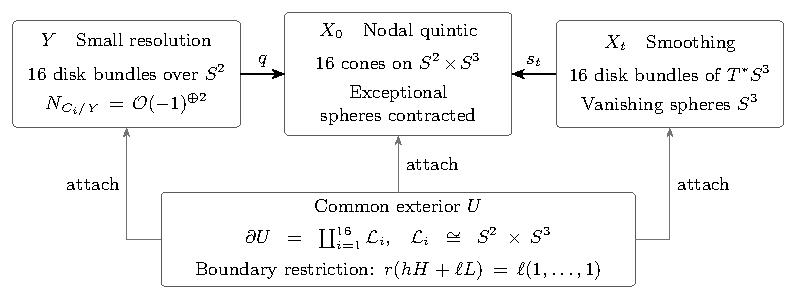
\includegraphics[width=\textwidth]{figures/output/fig01_transition.pdf}
 \caption{The common exterior and its three fillings. The map $q$ is
 algebraic; $s_t$ is the continuous Milnor collapse along the chosen ray.
 The resolution and smoothing cores have real dimensions two and three.
 The same boundary restriction gives the vanishing-cycle relation and
 the periods in the spectral coefficient.}
 \label{fig:transition}
\end{figure}

\subsection{The full integral rings}
Let $H,L$ be the hyperplane classes of $\PP^4,\PP^1$ restricted to $Y$.
Lefschetz gives $H_2(Y;\ZZ)=\ZZ^2$ and $H_2(X_t;\ZZ)=\ZZ$.
Together with $H_1=0$, universal coefficients and integral Poincar\'e
duality imply torsion-freeness in every degree. The fundamental class
of $Y$ in the product is $(H+L)(4H+L)$, whence
\begin{equation}\label{eq:split-cubic}
 \int_YH^3=5,\qquad \int_YH^2L=4,\qquad L^2=0.
\end{equation}
Take $A,B\in H^4(Y;\ZZ)$ dual to $H,L$, and let
$a_4\in H^4(X_t;\ZZ)$ satisfy $\int_{X_t}Ha_4=1$. Then:

\begin{table}[tb]
\centering
\caption{Integral cohomology and characteristic data of the compact fibres.}
\label{tab:integral-rings}
\begin{adjustbox}{max width=\textwidth,center}
\begin{tabular}{ll@{\hspace{1.5em}}l}
\toprule
 & $Y$ & $X_t$\\
\midrule
$H^2$ & $\ZZ H\oplus\ZZ L$ & $\ZZ H$\\
$H^4$ & $\ZZ A\oplus\ZZ B$ & $\ZZ a_4$\\
Degree-two products & $H^2=5A+4B$, $HL=4A$, $L^2=0$ & $H^2=5a_4$\\
Top products & $HA=LB=[\mathrm{pt}]$, $HB=LA=0$ & $Ha_4=[\mathrm{pt}]$\\
$\operatorname{rank}H^3$ & $174$ & $204$\\
$c_2$ & $50A+24B$ & $50a_4$\\
Euler characteristic & $-168$ & $-200$\\
\bottomrule
\end{tabular}
\end{adjustbox}
\end{table}

To verify the characteristic numbers directly, use
\[
 c(TY)=\frac{(1+H)^5(1+L)^2}{(1+H+L)(1+4H+L)}.
\]
This gives $c_2(Y)=6H^2+5HL$ and
$c_3(Y)=-20H^3-17H^2L$. For a quintic,
$c_2=10H^2$ and $c_3=-40H^3$. Since $H^1=H^5=0$, the Euler
numbers give the displayed third Betti numbers. The degree-three product
on each compact fibre is its unimodular alternating pairing times the
point class. With $H^0=H^6=\ZZ$, these statements specify the full rings
up to symplectic basis choices. The product subgroup generated by
$H^2$ and $HL$ in $H^4(Y)$ has index
$|\det\left(\begin{smallmatrix}5&4\\4&0\end{smallmatrix}\right)|=16$;
it is not an integral basis.

Every exceptional curve has degrees $(H\cdot C_i,L\cdot C_i)=(0,1)$.
They therefore represent the same primitive homology class $c_Y$, with
Poincar\'e dual $B$. Primitivity follows from the period of $L$.

\subsection{The common exterior and all cohomological attachments}
Remove disjoint tubular neighborhoods of the exceptional curves, obtaining
a compact exterior $U$. Its boundary components $\mathcal L_i$ are
$S^2\times S^3$. Define
\[
 \Lambda=\ZZ^{16},\quad \mathbf1=(1,\ldots,1),\quad
 \Lambda_0=\ker(\Sigma:\Lambda\to\ZZ),\quad W=\Lambda/\ZZ\mathbf1.
\]
The homological Thom sequence uses
$H_j(Y,U)=H_{j-4}(\coprod C_i)$.
The maps $H_4(Y)\to\Lambda$ and $H_6(Y)\to\Lambda$ have primitive
diagonal image: the former is exceptional intersection, witnessed by
$L\cdot C_i=1$, and the latter is the oriented diagonal fundamental
class. Thus $U$ has free integral homology and cohomology, with Betti
vector
\begin{equation}\label{eq:exterior-betti}
 (1,0,2,189,1,15,0),
\end{equation}
and exact sequences
\begin{equation}\label{eq:exterior-homology}
 0\to W\to H_3(U)\to H_3(Y)\to0,
 \qquad 0\to H_3(U)\to H_3(X_t)\to \Lambda_0\to0.
\end{equation}
The second comes from the Milnor fillings, whose cores are three-spheres.
The vanishing spheres span $W$, with relation
$\delta_1+\cdots+\delta_{16}=0$. Both successive quotients in
\eqref{eq:exterior-homology} are free; hence $W$ embeds primitively in
$H_3(X_t)$, and is isotropic because the spheres are disjoint.

In cohomology the Thom sequence kills exactly $\ZZ B$ in degree four.
Writing $\bar A=A|_U$, the even products are
\[
 H^2=5\bar A,\qquad HL=4\bar A,\qquad L^2=0.
\]
Orient each link as a boundary component of $U$ and choose generators
$\alpha_i\in H^2(\mathcal L_i)$ and $\beta_i\in H^3(\mathcal L_i)$
with $L|_{\mathcal L_i}=\alpha_i$ and $\int\alpha_i\beta_i=1$.
The symbol $\beta_i$ here has degree three; the harmonic degree-two
form remains $\vartheta_i$. The degree-three restriction is
\begin{equation}\label{eq:exterior-cohomology}
 0\to H^3(Y)\to H^3(U)\xrightarrow{r_U}\Lambda_0\to0,
\end{equation}
and degree-five restriction is the inclusion $H^5(U)=\Lambda_0\hookrightarrow\Lambda$.
Boundary multiplicativity and that injectivity imply, for $y\in H^3(U)$,
\[
 Hy=0,\qquad Ly=r_U(y)\in \Lambda_0=H^5(U).
\]
All degree-six products vanish. These formulas give the entire exterior
ring, without supplying an unspecified multiplication as additional input.

For completeness, use the Mayer--Vietoris difference $j_U^*-j_F^*$.
Let $x_i$ be the degree-two generator of the resolution filling and $z_i$
the degree-three generator of the smoothing filling, restricting to
$\alpha_i,\beta_i$. The nonzero difference maps are:
\begin{center}
\begin{adjustbox}{max width=\textwidth,center}
\begin{tabular}{cll}
\toprule
Degree & Resolution & Smoothing\\
\midrule
$0$ & $c_0\mathbf1-(c_i)$ & $c_0\mathbf1-(c_i)$\\
$2$ & $\ell\mathbf1-(x_i)$ & $\ell\mathbf1$\\
$3$ & $r_U(y)$ & $r_U(y)-(z_i)$\\
$5$ & $\Lambda_0\hookrightarrow\Lambda$ & $\Lambda_0\hookrightarrow\Lambda$\\
\bottomrule
\end{tabular}
\end{adjustbox}
\end{center}
Here $hH+\ell L$ is the exterior degree-two class, $c_0$ is an exterior
constant, and $(c_i)$ are filling constants.
The nonzero connecting maps are
\begin{equation}\label{eq:connecting-maps}
 \begin{aligned}
 \partial_Y^3(v)&=(\Sigma v)B,&
 \partial_Y^5(v)&=(\Sigma v)[\mathrm{pt}],\\
 \partial_{X_t}^2&:\Lambda\twoheadrightarrow W\hookrightarrow H^3(X_t),&
 \partial_{X_t}^5(v)&=(\Sigma v)[\mathrm{pt}].
 \end{aligned}
\end{equation}
All other connecting maps vanish. The signs follow by representing the
connecting class on an outward-$U$ collar by $d\chi_F\wedge\eta$,
where $\chi_F$ increases toward the filling. Pairing the degree-three
connecting class of $\beta_i$ with $H,L$ gives zero and one respectively,
hence $+B$. The same collar integral gives the top-degree sum maps.

Restriction from $Y$ preserves $H,L$, sends $(A,B)$ to $(\bar A,0)$,
and identifies $H^3(Y)$ with $\ker r_U$. Restriction from $X_t$ sends
$(H,a_4)$ to $(H,\bar A)$ and surjects $H^3(X_t)\to H^3(U)$ with
kernel the cohomological copy of $W$ in \eqref{eq:connecting-maps}.
Restriction to each Milnor filling is the corresponding component of
$r_U(y)$. These data specify the full integral cohomological attachment
diagram; no homotopy classification of the attaching maps is asserted.

\subsection{Monodromy and specialization}\label{sec:specialization}
Use left Poincar\'e duals in odd degree, characterized by
$\int\PD_L(\delta)\wedge\eta=\int_\delta\eta$, and orient $\delta_i$
so that $\PD_L(\delta_i)=\partial_{X_t}^2(\alpha_i)$.
For a positive simple loop, the Picard--Lefschetz transformation has
$N=T-I$, $N^2=0$, and, up to the common intersection-sign convention,
\begin{equation}\label{eq:monodromy}
 N\gamma=\pm\sum_{i=1}^{16}\langle\gamma,\delta_i\rangle\delta_i.
\end{equation}
Equivalently it factors through
$H_3(X_t)\to \Lambda_0\hookrightarrow\Lambda\twoheadrightarrow W$.
In the bases $e_i-e_{16}$ of $\Lambda_0$ and $\delta_1,\ldots,\delta_{15}$
of $W$, the nonzero block is $\pm(I_{15}+J_{15})$, where $J_{15}$
is the all-ones matrix. Its Smith form is
$\operatorname{diag}(1^{14},16)$: subtracting the first row from the
others gives fourteen unit pivots, and the remaining determinant is
sixteen. Thus the monodromy image has index sixteen in the primitive
vanishing lattice. This relation-matrix description is consistent with
the general conifold monodromy calculation of \cite{lee-lin-wang}.

The contraction $q:Y\to X_0$ collapses each exceptional sphere to its
node. Along the chosen smoothing ray, the Milnor collapse
$s_t:X_t\to X_0$ collapses each vanishing sphere. A disk cotangent bundle
of $S^3$ modulo its zero section is the cone on its sphere bundle; the
local collapses glue to the common exterior identification. Both maps
have degree one. Collapsing the sixteen cores to their distinct nodes
identifies the corresponding relative pairs with $(X_0,\{p_i\})$.
In degrees at least two its relative groups are $H_j(X_0)$. The pair
sequences give
\begin{equation}\label{eq:central-homology}
 \begin{split}
 &0\to H_3(Y)\xrightarrow{q_*}H_3(X_0)\to \Lambda_0\to0,\\
 &0\to W\to H_3(X_t)\xrightarrow{s_{t*}}H_3(X_0)\to0.
 \end{split}
\end{equation}
In degree two, $q_*$ is the quotient by $\ZZ c_Y$ and $s_{t*}$ is
an isomorphism. In degree four, $q_*$ is an isomorphism and $s_{t*}$
is a primitive injection with free rank-one cokernel. To see the latter,
the full relative sequence is
\[
 0\to H_4(X_t)\to H_4(X_0)\to\Lambda
 \xrightarrow{e_i\mapsto\delta_i}H_3(X_t)\to H_3(X_0)\to0,
\]
and the middle kernel is $\ZZ\mathbf1$. All central groups are free,
with Betti vector $(1,0,1,189,2,0,1)$. The maps are isomorphisms in
degrees zero and six; degrees one and five vanish.

The first sequence of \eqref{eq:exterior-homology} maps to the second
sequence of \eqref{eq:central-homology}, with identity on $W$, exterior
inclusion in the middle, and $q_*$ on the right. Both vertical cokernels
are canonically $\Lambda_0$. This is naturality of the actual collapse maps,
rather than an arbitrary splitting of free groups.

Let $h\in H^2(X_0)$ be the central polarization and choose
$A_0,B_0\in H^4(X_0)$ by $q^*(h,A_0,B_0)=(H,A,B)$.
The central even products and smoothing pullback are
\begin{equation}\label{eq:central-ring}
 h^2=5A_0+4B_0,\quad hA_0=[\mathrm{pt}],\quad hB_0=0,
 \qquad s_t^*(h,A_0,B_0)=(H,a_4,0).
\end{equation}
Indeed pairing the degree-four pullbacks with $H$, and using degree one,
fixes their coefficients integrally. Dually the image of $s_{t*}$ in
degree four is $\ZZ q_*\PD_Y(H)$. In degree three $q^*$ is surjective
with primitive kernel $\Lambda_0^*\simeq W$, and $s_t^*$ is a primitive injection
onto the annihilator of the vanishing homology lattice. Since $\im N$
has finite index in $W$, an integer-valued homomorphism annihilates
$\im N$ exactly when it annihilates $W$. Thus
\[
 \im s_t^*=\ker(T^*-I)\subset H^3(X_t;\ZZ).
\]
The central degree-three cup pairing factors through $q^*$ and the
unimodular pairing of $Y$, by naturality and degree one. Its radical is
$\ker q^*$; the Milnor pullback takes that radical to the primitive
vanishing cohomology lattice by naturality of the connecting map.
These formulas specify the central ring, including its degenerate
middle pairing, without assuming ordinary Poincar\'e duality for $X_0$.

\subsection{The spectral coefficient and the allowed parameters}
Proposition~\ref{prop:split-existence} and Table~\ref{tab:integral-rings}
verify all hypotheses of Theorem~\ref{thm:main}. Taking $D=L$ gives
\[
 M=\frac{4^2}{5}-0=\frac{16}{5},\qquad
 \frac{2\pi\sum_{i=1}^{16}(L\cdot C_i)^2}{M}=10\pi,
\]
which proves the spectral assertion of Theorem~\ref{thm:integrated}.
By Proposition~\ref{prop:restriction-spectrum}, the vector
$(L\cdot C_i)_i=\mathbf1$ in this calculation is the same vector
that generates the kernel of the vanishing-cycle map. The denominator
is the polarized primitive norm from the same integral ring. It is
not an independent local coefficient fitted to the spectrum.

The family has one exceptional-area direction. Arbitrary independent
node parameters are not implied by the number of nodes. Already at
first order, evaluation of quintics at the sixteen planar points has
rank fifteen: the degree-five Hilbert function of a plane $(4,4)$
complete intersection is $\binom72-2\binom32=15$.
Cayley--Bacharach makes the unique evaluation relation nonzero at every
point. The actual pencil selects a compatible vector nonzero at all
nodes. This is sufficient for the fixed-ray theorem and does not
supply uniformity for arbitrary independent smoothing rates.

\section{Tangent sheaves and Hermitian--Einstein limits}\label{sec:tangent}

The tangent bundles provide compatible nontrivial holomorphic data on the
same transition. Their Hermitian--Einstein connections are intrinsic to
the Ricci-flat metrics, but their algebraic extensions across the central
fibre require a separate calculation. We make that distinction explicit.

\subsection{The flat limit and its reflexive hull}
For the family \eqref{eq:split-equations}, put
\[
 \mathcal A=T_{\PP^4}|_{\mathcal X},\qquad
 \mathcal B=\OO_{\mathcal X}(5),\qquad
 \mathcal K=\ker(\mathcal A\xrightarrow{d_{\PP^4}(F_0+tG)}\mathcal B).
\]
Thus $\mathcal K=T_{\mathcal X/\Delta}$, and set
$E_0=\mathcal K|_{X_0}$. Write $Q=\bigoplus_{i=1}^{16}\CC_{p_i}$.

\begin{proposition}\label{prop:tangent-sheaf}
The sheaf $\mathcal K$ is flat over the disc and restricts to $T_{X_t}$
for $t\ne0$. There are identities and an exact sequence
\begin{equation}\label{eq:tangent-specialization}
 0\to E_0\to T_{X_0}\to Q\to0,\qquad
 E_0^{**}=T_{X_0},\qquad q_*T_Y=T_{X_0},\qquad
 R^jq_*T_Y=0\quad(j>0).
\end{equation}
At each node $T_{X_0}$ is reflexive of depth two, whereas $E_0$ has
depth one and is not reflexive. On each exceptional curve,
\begin{equation}\label{eq:tangent-splitting}
 T_Y|_{C_i}=\OO(2)\oplus\OO(-1)^{\oplus2}.
\end{equation}
\end{proposition}
\begin{proof}
Let $\mathcal I$ and $\mathcal Q$ be the image and cokernel of the
relative Jacobian map. Locally the total space is smooth and the
projection has equation $\sum z_j^2=t$. Hence $\mathcal Q$ is a
length-one skyscraper at each node, annihilated by $t$, and vanishes
elsewhere near the central fibre. Both $\mathcal I\subset\mathcal B$
and $\mathcal K\subset\mathcal A$ have no base-parameter torsion,
so they are flat over the smooth one-dimensional base. Tensor the
sequences
\[
 0\to\mathcal K\to\mathcal A\to\mathcal I\to0,
 \qquad 0\to\mathcal I\to\mathcal B\to\mathcal Q\to0
\]
with the central fibre. The first stays left exact, and the second
gives $\ker(\mathcal I_0\to\mathcal B_0)=
\operatorname{Tor}_1^{\OO_\Delta}(\mathcal Q,\CC)=Q$.
The kernel of $\mathcal A_0\to\mathcal B_0$ is $T_{X_0}$, so the
snake lemma gives the first sequence in \eqref{eq:tangent-specialization}.

At a node let $R=\CC\{z_1,\ldots,z_4\}/(\sum z_j^2)$ and let
$\mathfrak m$ be its maximal ideal. The tangent module is the kernel
of $R^4\to\mathfrak m$. The sequence
$0\to\mathfrak m\to R\to\CC\to0$ gives depth one for $\mathfrak m$,
and the kernel consequently has depth two. It is torsion-free and
locally free off the node, hence reflexive on this normal threefold.
The sequence with nonzero length-one quotient then gives depth one
for $E_0$. Both sheaves agree off codimension three, so their reflexive
hulls agree.

The exceptional locus in the smooth $Y$ has complex codimension two. Holomorphic sections of its tangent bundle extend
across those curves. On the common regular locus this identifies
$q_*T_Y$ with the reflexive extension $T_{X_0}$
\cite[Tags 0EBJ and 0AY6]{stacks}.
For the higher direct images, the tangent-normal sequence over $C_i$
splits because $H^1(\PP^1,\OO(3))=0$, giving
\eqref{eq:tangent-splitting}. If $I$ is the exceptional ideal,
$I^n/I^{n+1}=\OO(n)^{\oplus(n+1)}$. Tensoring with the tangent
restriction gives degrees $n+2$ and $n-1$, whose first cohomology
vanishes for every $n\ge0$. Induction through the thickening sequences
therefore gives $H^1(T_Y/I^{n+1}T_Y)=0$.
In an incidence chart the node coordinates are the entries of
$\left(\begin{smallmatrix}a&b\\ua&ub\end{smallmatrix}\right)$;
the pulled-back node ideal is $(a,b)=I$. These are exactly the
thickenings required by formal functions, not merely an equivalent
informal neighborhood model. Formal functions and faithful flatness
of completion give $R^1q_*T_Y=0$ \cite[Tag 02OC]{stacks}.
The fibres have dimension at most one, so all higher direct images
vanish as well.
\end{proof}

The exceptional splitting rules out locally free descent across the
contracted point. In particular the resolution direct image is the
reflexive hull, not the flat central fibre $E_0$. Compatibility is
through the common regular tangent bundle and the specified coherent
extensions. The exterior identifications on the smoothing side are
differentiable, not generally biholomorphic. No single flat family
containing both the resolution and smoothing branches is asserted.

Every smooth deformation has its intrinsic relative tangent bundle.
Thus this bundle choice introduces no additional existence obstruction
on smooth base deformations. The singular flatness calculation above
uses the actual one-dimensional family with nonzero linear local
smoothing terms. It is not a flatness theorem over an arbitrary
higher-dimensional singular deformation base. As a consistency check,
proper flatness, \eqref{eq:tangent-specialization} and the direct images
imply the holomorphic Euler-characteristic identity
$\chi(Y,T_Y)-\chi(X_t,T_{X_t})=16$, distinct from the topological
Euler-characteristic difference $32$.

\subsection{Actual metrics and controlled local curvature}
On the resolution use the K\"ahler class $H+\epsilon^2L$, the restriction
of a positive product class, and on the smoothing use $H$ with
$t=\epsilon^3$. Denote either branch by $Z_\epsilon$, with its actual
Ricci-flat metric $g_\epsilon$.

\begin{proposition}\label{prop:tangent-metrics}
The nontrivial tangent bundles $T_Y$ and $T_{X_t}$ are stable for these
classes. Their Ricci-flat tangent connections are irreducible zero-slope
Hermitian--Einstein connections. Both branches converge to the same
metric completion $(X_0,d_{g_0})$, homeomorphic to $X_0$, smoothly on
fixed regular compact subsets. Near each node, after rescaling by
$\epsilon^{-2}$, the metrics and tangent connections converge with all
derivatives to the normalized nonflat resolved-conifold or Stenzel
model.

For each node there is a collar radius $r$, extended over the cap with
$r+\epsilon\asymp\epsilon$ there, and fixed constants such that
\begin{equation}\label{eq:tangent-bounds}
 \begin{aligned}
 |\nabla^j\Rm(g_\epsilon)|&\le C_j(r+\epsilon)^{-2-j},\qquad j\ge0,\\
 \vol\{r<\rho\}&\le C\rho^6,\qquad
 \int_{\{r<\rho\}}|F_{T_{Z_\epsilon}}|^2dV\le C\rho^2,
 \qquad \epsilon\le\rho\le\rho_0,\\
 d_{GH}((Z_\epsilon,g_\epsilon),(X_0,d_{g_0}))&\le C\epsilon^\theta
 \quad\text{for some }\theta>0.
 \end{aligned}
\end{equation}
All tensor norms, derivatives and volumes in this display use the actual
metric. In particular the unscaled tangent curvature-energy measure has
no atom at a node.
\end{proposition}
\begin{proof}
Existence of the smooth Ricci-flat metrics is Yau's theorem \cite{yau}.
The holonomy argument following \eqref{eq:central-cohomology} gives
full $\mathrm{SU}(3)$. Ricci-flatness makes the tangent connection
Hermitian--Einstein of zero slope; irreducibility and the
Hermitian--Einstein stability implication give stability
\cite[Theorem~5.8.3]{kobayashi}. These bundles are nontrivial since their
second Chern pairing with $H$ is $50$.

The actual smoothing expansion was verified in
Proposition~\ref{prop:metric-comparison}. On the resolution all local
areas are $\int_{C_i}(H+\epsilon^2L)=\epsilon^2$. Thus the local AC
K\"ahler classes lie in the restriction image of the single global
class $L$, exactly Assumption R of Benabida's Theorem~B
\cite{benabida}; his Example~1.5 also treats this split quintic.
The face restrictions give the claimed central and rescaled local
limits, with all derivatives. For tangent connections these follow
by differentiation of the actual metrics and complex structures.

The positive face metrics and the bounded differentiated coefficients
in conic frames give uniform cone comparison on annuli and scaled
AC comparison on the core. Every physical derivative costs
$(r+\epsilon)^{-1}$; two derivatives give curvature. This proves the
first line of \eqref{eq:tangent-bounds} and core volume $O(\epsilon^6)$.
Integrating the annular volume comparison gives the displayed
$C\rho^6$ bound. On a dyadic annulus of radius $s\ge\epsilon$,
the tangent curvature energy is bounded by $Cs^{-4}s^6=Cs^2$.
Summing to the core, whose energy is $O(\epsilon^2)$, gives $C\rho^2$.
The central cone comparison adds one point in the metric completion
at each node and identifies its topology with the algebraic cone,
so the completion is homeomorphic to $X_0$.

We give the global distance estimate explicitly. Each filled region
$\{r<\rho\}$ has intrinsic diameter at most $C\rho$: radial annular
lengths sum to $O(\rho)$, fixed-radius links have diameter $O(\rho)$,
and the core has diameter $O(\epsilon)$. Collapsing the sixteen
regions to points changes Gromov--Hausdorff distance by at most
$C\rho$. Indeed a shortest quotient chain need visit each collapsed
point at most once, and each jump can be replaced by a path of its
intrinsic diameter. The same applies to the central space. On the
common exterior the actual tensor comparison, and its resolution
analogue from Theorem~B, give relative error $O((\epsilon/\rho)^{a_0})$.
The resulting quotient spaces have uniformly bounded diameter and
are bilipschitz with factor $1+O((\epsilon/\rho)^{a_0})$.
Consequently
\[
 d_{GH}(Z_\epsilon,X_0)\le C\bigl(\rho+(\epsilon/\rho)^{a_0}\bigr).
\]
Taking $\rho=\epsilon^{a_0/(1+a_0)}$ proves the last line of
\eqref{eq:tangent-bounds}, with a possibly smaller common exponent
for the two branches.
\end{proof}

The energy statement allows nonflat rescaled limits and unbounded
pointwise curvature. It supplies neither uniform estimates for arbitrary
gauge bundles nor a theorem for their HYM flows. Its role here is to
identify the actual tangent geometry compatible with the explicitly
calculated transition.

\subsection{Proof of the integrated theorem}
\begin{proof}[Proof of Theorem~\ref{thm:integrated}]
Proposition~\ref{prop:split-existence} establishes the genuine projective
family, the chosen resolution and the smooth fibres. The complete
intersection calculation in Section~\ref{sec:quintic} gives the
torsion-free smooth rings, their Chern classes and pairings. The Thom
and Mayer--Vietoris calculations there determine the exterior ring and
all cohomological attachments. The contraction and Milnor collapse
give the central ring and specialization maps by the relative pair
sequences, with the naturality described in
Section~\ref{sec:specialization}. This proves part~(1).

Use the collar-compatible trivialization of
Proposition~\ref{prop:metric-comparison} as the exterior identification
in the attachment calculation. Its horizontal lift agrees with the
prescribed node collars and is defined over the fixed ray. Two such
extensions away from the collars are isotopic along that ray, so they
induce the same marked cohomology maps. Thus the analytic and
topological link generators can be chosen identically.
Proposition~\ref{prop:restriction-spectrum} gives
\eqref{eq:split-exact-sequence}, since the hyperplane class $H$ is
primitive on the smooth quintic and $r(L)=\mathbf1$.
The freeness of $H^3(U;\ZZ)$ makes its vanishing sublattice primitive.
The disjoint vanishing spheres make it isotropic. The calculated
factorization $\Lambda_0\hookrightarrow\Lambda\twoheadrightarrow W$ gives
the displayed Picard--Lefschetz block and its Smith form, proving
part~(2).

For part~(3), the same integral class $L$ has
$L\cdot C_i=1$ and cubic data $(H^3,LH^2,L^2H)=(5,4,0)$.
It determines the exceptional areas $s^2$ in class $H+s^2L$.
On the central regular locus, Proposition~\ref{prop:mass} represents
$L-4H/5$ by the primitive harmonic form of squared norm $16/5$.
Identity~\eqref{eq:period-capacity-identification} identifies its
sixteen boundary coefficients with the same $r(L)=\mathbf1$.
The spectral theorem therefore gives $10\pi$, with its stated
count, type and error. Proposition~\ref{prop:tangent-metrics}
supplies the actual metric limits on the two branches. Apply its
resolution assertion with $\epsilon=s$ and its smoothing assertion
with $\epsilon=t^{1/3}$ separately; no ratio of $s$ and $t$ is used.

Finally, Proposition~\ref{prop:tangent-sheaf} identifies the flat
central tangent sheaf and its distinct reflexive hull, and
Proposition~\ref{prop:tangent-metrics} proves the tangent stability
and actual connection limits. This proves part~(4). These statements
use the same central regular tangent bundle; they do not identify
the flat central sheaf with the resolution direct image, or assert a
flat family containing both branches. The restriction, primitive norm
and actual collar identifications above provide the compatibility
between the topological and analytic assertions.
\end{proof}

\section{The eight-node transition and its two small modes}\label{sec:eight-node}

We apply Theorem~\ref{thm:matrix} to the compact transition constructed
in stability--degeneration Paper~2,
\cite[Appendix~A, Proposition~A.1]{wuebben-chambers}. This uses its
geometric realization and exceptional-curve data as premises. The
additional deformation argument below supplies a polarized smoothing
with the precise first-order and canonical-bundle properties required
by the analytic theorem.
This family has dual-edge length four at its nontriangular toric faces;
it is outside the length-one admissible class of CY~VI
\cite[Definition~2.1]{wuebben-cy-mirror}.

\subsection{A polarized simple smoothing of the earlier example}
Let $B=\PP^1\times\PP^1$, $L=\OO_B(1,-1)$, and
\begin{equation}\label{eq:eight-ambient}
 Z=\PP_B(\OO\oplus L)\times_B\PP_B(\OO\oplus L).
\end{equation}
Use the quotient convention for the tautological classes $\xi_1,\xi_2$,
and write $f,g$ for the base hyperplane classes. Let $\bar Z$ be the
anticanonical model, $Y\subset Z$ a general anticanonical hypersurface
chosen simultaneously nondegenerate for its toric polytope, and
$q:Y\to X_0\subset\bar Z$ the induced contraction. Set
\begin{equation}\label{eq:eight-polarization}
 \mathcal L_0=(-K_{\bar Z})|_{X_0},\qquad
 H=c_1(q^*\mathcal L_0)=(4g+2\xi_1+2\xi_2)|_Y.
\end{equation}

\begin{proposition}\label{prop:eight-family}
The threefold $X_0$ has eight ordinary double points and the displayed
map is a smooth simply connected projective small crepant resolution.
There is a proper flat projective smoothing over a disc, with trivial
relative canonical bundle and a relatively ample line bundle restricting
to the exact $\mathcal L_0$, such that every local smoothing function
has nonzero first derivative. The smooth fibres are simply connected,
and the second Betti numbers of $Y$ and $X_t$ are four and two.
\end{proposition}
\begin{proof}
The cited construction proves that $\bar Z$ has two disjoint singular
projective lines with transverse ordinary-node singularities. A general
anticanonical section meets each in four simple points. Its projective
crepant toric refinement restricts to $q$, and the resulting smooth
$Y$ has Hodge pair $(4,60)$, trivial canonical bundle and
$H^1(\OO_Y)=H^2(\OO_Y)=0$. Rationality of the nodes transfers both
vanishings to $X_0$. The model $\bar Z$ is Gorenstein Fano, so
$\mathcal L_0$ is ample and Cartier. The canonical-class calculation
in the quotient convention gives \eqref{eq:eight-polarization}, and
Cartier adjunction gives $\omega_{X_0}\simeq\OO_{X_0}$.

The four-plus-four multiplicity and the curve periods can also be read
directly from the bundle construction. Let $S_f,S_g\simeq B$ be the
sections for which both quotients are respectively onto $\OO$ and onto
$L$. Their normal bundles and anticanonical restrictions are
\[
 N_{S_f/Z}=(L^{-1})^{\oplus2},\quad N_{S_g/Z}=L^{\oplus2},\qquad
 (-K_Z)|_{S_f}=\OO(0,4),\quad (-K_Z)|_{S_g}=\OO(4,0).
\]
The restrictions of global sections are complete linear systems: the
all-$\OO$ and all-$L$ summands in
\[
 \pi_*\OO_Z(-K_Z)=\OO(0,4)\otimes\operatorname{Sym}^2(\OO\oplus L)
                              \otimes\operatorname{Sym}^2(\OO\oplus L)
\]
have independent coefficients. A general section therefore meets each
$S$ in four distinct fibres of its contracted ruling. For one such fibre
$C$, the sequence with $N_{C/S}=\OO$ and $N_{S/Z}|_C=\OO(-1)^{\oplus2}$
splits, since $H^1(\PP^1,\OO(1))=0$. The normal derivative of the
anticanonical equation is an isomorphism on the trivial summand because
the corresponding quartic zero is simple. Hence
$N_{C/Y}=\OO(-1)^{\oplus2}$. The divisor degrees in the basis
$(f,g,\xi_1,\xi_2)$ are
\begin{equation}\label{eq:eight-period-types}
 \Gamma_f=(1,0,0,0),\qquad \Gamma_g=(0,1,-1,-1).
\end{equation}
The imported global contraction calculation excludes further exceptional
loci or singularities, and its Picard-rank computation shows that these
four divisor classes span $H^2(Y;\QQ)$. Thus the displayed degrees
determine the rational exceptional homology classes.
Its full rational relation space is given by separate sum-zero
conditions on these two groups of four. In particular
$(1,1,1,-3;1,1,1,-3)$ has full support.
The first-order criterion of
\cite[Theorem~1.2 and Section~3, (3.2)]{rollenske-thomas} gives a
deformation tangent nonzero in every local node-smoothing space.
Theorem~1.6 of \cite{friedman-unobstructed} makes this tangent
unobstructed: $X_0$ is a compact Gorenstein Calabi--Yau threefold,
its isolated rational lci singularities are Du~Bois, its projective
resolution satisfies the $\partial\bar\partial$ lemma, and
$H^1(\OO_{X_0})=0$.

We verify projective effectivity and the exact polarization.
Choose $N$ so that $\mathcal L_0^N$ is very ample and
$H^1(\mathcal L_0^N)=0$. Over a small Artin extension, the
vanishing of $H^2(\OO_{X_0})$ lifts the embedding line bundle,
and $H^1(\mathcal L_0^N)=0$ lifts its coordinate sections.
The lifted morphism remains a closed immersion over the nilpotent
thickening. Thus embedded deformations map formally smoothly to
abstract deformations; equivalently the restricted Euler sequence
gives $H^1(T_{\PP^M}|_{X_0})=0$.
The corresponding Hilbert-scheme germ is smooth. Retain a lift of the
selected tangent and shrink to a neighbourhood $S$ with integral fibres.

Perform the Picard construction over this scheme $S$ before choosing
the analytic disc. After an \'etale neighbourhood, the universal family
has a section through a smooth point of $X_0$
\cite[Tag~055S]{stacks}. Its proper integral fibres give the universal
identity $\OO_T\simeq p_{T*}\OO$ under base change, where $p$ is the universal family projection.
The relative Picard scheme exists, and the section supplies a universal
Poincar\'e line bundle, normalized along that section
\cite[Theorems~2.5(2), 4.8; Exercises~3.11, 4.3 and their Appendix~A
solutions]{kleiman-picard}. Since $H^2(\OO_{X_0})=0$, the Picard
morphism is smooth at $[\mathcal L_0]$
\cite[Proposition~5.19]{kleiman-picard}. A further \'etale
neighbourhood gives a section through this point; pulling back the
Poincar\'e bundle extends precisely $\mathcal L_0$.
Ampleness is open. Both base changes have isomorphic tangent maps at
the chosen complex points. A holomorphic disc in the resulting smooth
base with the prescribed tangent therefore gives a relatively polarized
projective family and retains every nonzero local derivative. No
ramified reparametrization or replacement of $H$ by $NH$ occurs.

At a node the local equation is
$\sum z_j^2=\tau_i(t)$ with $\tau_i'(0)\ne0$, so the total
space is smooth. Properness allows the disc to be shrunk so that
the entire total space is smooth and the family is Gorenstein.
Its relative dualizing line bundle restricts to
$\omega_{X_0}\simeq\OO_{X_0}$. Since
$H^1(\omega_{X_0})=0$, cohomology and base change lifts a central
nowhere-zero generator to a relative section. Its zero set has proper
image missing the origin. Shrinking the disc removes that image and
trivializes the actual relative canonical bundle.

For simple connectivity, apply
\cite[Corollary~1.9]{batyrev-kreuzer} to the nondegenerate toric
hypersurface and the smooth projective crepant subdivision in the
construction. Its lattice quotient is zero: the relevant dual-polytope
vertices include the lattice basis $e_1,e_2,f_0,g_0$.
Thus $\pi_1(Y)=0$. The common exterior has simply connected links
$S^2\times S^3$, and the two kinds of filling retract onto $S^2$
and $S^3$. Van Kampen gives $\pi_1(X_t)=\pi_1(Y)=0$.
Finally the two independent exceptional classes give
$b_2(X_t)=4-2=2$, as also computed in the earlier proposition.
\end{proof}

These properties verify the general smoothability hypothesis of
Hein--Sun and the smoothing hypotheses of Benabida used in
Section~\ref{sec:geometry}. Locally write $\tau_i(t)=t u_i(t)$
with $u_i(0)\ne0$; a holomorphic square root of $u_i$ changes the
coordinates to the model $\sum z_j^2=t$ over the same base.
The Stenzel metric supplies the exact affine K\"ahler model. The
finite-node construction has fixed positive leading scale ratios,
and neither metric theorem imposes $b_2(X_t)=1$.
In particular the actual metrics in class $H$ satisfy the comparisons
used in Theorem~\ref{thm:matrix}.

\subsection{The quotient mass and the two coefficients}
The earlier construction calculates
\begin{equation}\label{eq:eight-intersection}
 \left(\int_YD_iD_jH\right)_{i,j}
 =\begin{pmatrix}
 0&8&4&4\\8&0&12&12\\4&12&-8&0\\4&12&0&-8
 \end{pmatrix},\qquad (D_i)=(f,g,\xi_1,\xi_2).
\end{equation}
It follows directly from
$f^2=g^2=0$, $\xi_i^2=(f-g)\xi_i$ and
$\int_Zfg\xi_1\xi_2=1$, by integrating $D_iD_j(-K_Z)^2$;
the same calculation gives $H^3=320$.
The restriction kernel has basis
\[
 k_1=g+\xi_1,\qquad k_2=g+\xi_2,
 \qquad H=2k_1+2k_2.
\]
Choose quotient lifts $f,g$. By \eqref{eq:eight-period-types}, their
period vectors have disjoint four-entry unit supports. The energy
matrix is $\mathsf E=4I_2$. The intersection blocks are
\[
 B_{KK}=\begin{pmatrix}16&24\\24&16\end{pmatrix},\quad
 B_{DK}=\begin{pmatrix}12&12\\12&12\end{pmatrix},\quad
 B_{DD}=\begin{pmatrix}0&8\\8&0\end{pmatrix}.
\]
Consequently \eqref{eq:mass-schur} gives
\begin{equation}\label{eq:eight-mass}
 \mathsf M=\frac45\begin{pmatrix}9&-1\\-1&9\end{pmatrix}.
\end{equation}
The orthogonal primitive lifts
\[
 D_-=f-g,\qquad D_+=f+g-\frac35(k_1+k_2)
\]
have squared masses $16$ and $64/5$, respectively, and both have
squared period norm $8$. Thus the generalized eigenvalues of
$(\mathsf E,\mathsf M)$ are $1/2$ and $5/8$.
Theorem~\ref{thm:matrix} proves \eqref{eq:eight-spectral-law},
including the count, eventual simplicity, type and gaps, and completes
the proof of Corollary~\ref{cor:eight-node}.

Only rational divisor data are used here. No new integral basis,
saturation or full cohomology-ring assertion is made for this family.
The application uses the earlier compact construction to derive new
information about its actual metric operators. It preserves the
distinction established there between tangent-stability walls in the
ambient fourfold, toric contraction circuits and Calabi--Yau cycle
relations.

\section{Three small modes on a four-node toric transition}\label{sec:cy-x9}

We now use the original-side nodal partial resolution $X'_9$ constructed
in CY~VI \cite[Section~11.1 and Appendix~G.1]{wuebben-cy-mirror}.
That paper supplies its four nodes, a projective small resolution and
the integral exceptional-curve relation. The deformation results of
CY~V supply a prescribed first-order smoothing tangent and its
integrability. We specify an exact polarization, verify the remaining
family hypotheses, and compute three spectral coefficients from the
full quotient harmonic norm. This connects the earlier geometric
construction to Theorem~\ref{thm:matrix}.

The notation distinguishes three spaces. The original $X_9$ of CY~V
has two nodes and a degree-seven del Pezzo cone; it does not satisfy
our nodal hypotheses. Its partial resolution $X'_9$ has four nodes.
The four-node mirror studied elsewhere in CY~VI is a different
threefold. Only $X'_9$ is used in this section.

\subsection{The earlier nodal model and its polarization}
The eleven rays $v_0,\ldots,v_{10}$ of the original-side ambient fan
are the columns of
\begin{equation}\label{eq:x9-rays}
 \begin{pmatrix}
 1&0&-1&0&0&-4&-4&3&2&-1&-2\\
 0&1&-1&0&0&-2&-2&1&1&0&-1\\
 0&0&0&1&0&-1&0&1&1&0&0\\
 0&0&0&0&1&0&-1&1&1&0&0
 \end{pmatrix}.
\end{equation}
The first nine are the vertices of the reflexive polytope $\Delta_9$;
$v_9$ is interior to a facet and $v_{10}$ is the pentagon centre.
Use the source's integral support vector
\begin{equation}\label{eq:x9-height}
 h=(2,2,2,3,3,3,3,2,2,1,2),\qquad
 P_h=\{u\in\RR^4:h_i+\langle u,v_i\rangle\ge0\text{ for all }i\}.
\end{equation}
Its normal fan is the source fan $\Sigma'$ with twenty-one maximal
cones. The vertices of $P_h$ are
\begin{equation}\label{eq:x9-cartier-vertices}
\begin{array}{rrr}
(-2,-2,-3,15)&(-2,-2,-3,9)&(-2,-2,15,-3)\\
(-2,-2,9,-3)&(-2,-2,15,15)&(-2,4,-3,3)\\
(-2,4,3,-3)&(-2,4,3,3)&(1,-2,-3,3)\\
(0,-2,-3,3)&(1,-2,-3,1)&(1,-2,3,-3)\\
(0,-2,3,-3)&(1,-2,1,-3)&(1,-2,3,3)\\
(0,2,-3,-1)&(0,2,-1,-3)&(0,2,-1,-1)\\
(1,0,-3,-1)&(1,0,-1,-3)&(1,0,-1,-1).
\end{array}
\end{equation}
Substitution in \eqref{eq:x9-height} gives the source cones as the
active sets; every omitted inequality has margin at least one.
The recession cone is zero: pairing with $v_0,v_1,v_2$ first forces
the first two coordinates to vanish, and the remaining opposite
coordinate pairs force the other two to vanish. Thus these integral
vertices give a strictly convex Cartier support function. On
$P'=X_{\Sigma'}$, the divisor $A=\sum h_iD_i$ is ample and Cartier.
Set
\begin{equation}\label{eq:x9-polarization}
 \mathcal L_0=A|_{X'_9},\qquad H=c_1(q^*\mathcal L_0).
\end{equation}
Here $X'_9$ is the proper transform of a sufficiently general
nondegenerate anticanonical member for $\Delta_9$.

For an explicit smooth ambient refinement, replace the heights by
\begin{equation}\label{eq:x9-fine-height}
 a_i=h_i-\frac{\mathbf1_{i=3}+\mathbf1_{i=4}}{100}
             +\frac{i^2}{10^6}.
\end{equation}
The maximal cones of the normal fan of $P_a$ have ray-index sets
\begin{equation}\label{eq:x9-fine-fan}
\begin{gathered}
\{0,1,3,6\},\ \{0,1,3,7\},\ \{0,1,4,5\},\ \{0,1,4,7\},\\
\{0,1,5,6\},\ \{0,2,3,6\},\ \{0,2,3,7\},\ \{0,2,4,5\},\\
\{0,2,4,7\},\ \{0,2,5,6\},\ \{1,3,6,9\},\ \{1,3,7,8\},\\
\{1,3,8,9\},\ \{1,4,5,9\},\ \{1,4,7,8\},\ \{1,4,8,9\},\\
\{1,5,6,9\},\ \{2,3,6,10\},\ \{2,3,7,8\},\ \{2,3,8,10\},\\
\{2,4,5,10\},\ \{2,4,7,8\},\ \{2,4,8,10\},\ \{2,5,6,10\},\\
\{3,6,9,10\},\ \{3,8,9,10\},\ \{4,5,9,10\},\ \{4,8,9,10\},\\
\{5,6,9,10\}.
\end{gathered}
\end{equation}
Each ray matrix has determinant $\pm1$, and each cone lies in a cone
of $\Sigma'$ and in a facet of $\Delta_9$. Consequently its toric
fourfold $T$ is smooth and projective and the refinement is crepant.
At the four source parallelograms
\begin{equation}\label{eq:x9-nodes}
 q_1=(3,6,10,8),\quad q_2=(2,6,3,7),\quad
 q_3=(4,5,10,8),\quad q_4=(2,5,4,7),
\end{equation}
the refinement uses the diagonal $\{a,c\}$ of $q=(a,b,c,d)$.
Thus the anticanonical proper transform $Y\subset T$ is the source's
chosen projective small resolution $q:Y\to X'_9$.
Extra refinements over facet-interior strata do not change the
hypersurface: those strata map to torus-fixed points missed by a
nondegenerate member. In particular the additional nonsimplicial
coarse cone with rays $\{2,7,8,10\}$ is contained in a single original
facet and contributes no fifth node. These model identifications use
\cite[Proposition~3.4]{wuebben-cy-mirror}.

\subsection{A first-order family with the prescribed ample class}
We state explicitly the additional deformation step. The nodal
specializations of CY~V used here formulate the classical criterion;
no mixed-cone extension of the spectral theorem is asserted.

\begin{lemma}\label{lem:polarized-nodal-family}
Let $Z$ be a connected normal projective nodal threefold over $\CC$
with $\omega_Z\simeq\OO_Z$ and
$H^1(\OO_Z)=H^2(\OO_Z)=0$, admitting a projective small crepant
resolution. Suppose the exceptional-curve relation space contains a
vector with no zero coordinate. For every ample Cartier line bundle
$\mathcal L_0$ on $Z$, there is a proper flat projective smoothing
over a disc, with trivial relative canonical bundle and a relatively
ample line bundle restricting to exactly $\mathcal L_0$, such that
every node is smoothed to first order.
\end{lemma}
\begin{proof}
By \cite[Theorem~2.5]{wuebben-cy-smoothing}, the full-support relation
lifts to a global deformation tangent whose image in every local
node-smoothing space is nonzero. The common-volume-form
identifications may rescale equation parameters by nonzero factors,
which preserve this condition. The deformation base is smooth by
\cite[Theorem~4.5]{wuebben-cy-smoothing}; its additional degree-six
hypothesis is vacuous for nodes.

The projective effectivity construction in
Proposition~\ref{prop:eight-family} applies with this chosen tangent.
For completeness, choose $N$ with $\mathcal L_0^N$ very ample and
$H^1(\mathcal L_0^N)=0$. Across a small Artin extension, the
obstruction to lifting this line bundle lies in $H^2(\OO_Z)$ and
the obstruction to lifting its coordinate sections lies in
$H^1(\mathcal L_0^N)$. Both vanish. The lifted map remains a closed
immersion. Embedded deformations therefore map formally smoothly to
abstract deformations, and the Hilbert germ is smooth with a lift of
the selected tangent.

Work on a finite-type Hilbert neighbourhood with integral fibres.
An \'etale neighbourhood supplies a section through a smooth point of
$Z$ \cite[Lemma~37.38.5, Tag~057G]{stacks}. The relative Picard
scheme and its normalized Poincar\'e bundle then exist as in
\cite[Theorems~2.5(2), 4.8 and Exercise~4.3]{kleiman-picard}.
The Picard morphism is smooth at $[\mathcal L_0]$ because
$H^2(\OO_Z)=0$ \cite[Proposition~5.19]{kleiman-picard}.
A further \'etale-local section through that point extends
$\mathcal L_0$ itself. Ampleness persists after shrinking.
Both changes of base induce tangent isomorphisms. A disc with the
chosen tangent in the resulting smooth base retains every nonzero
local derivative. The auxiliary power $N$ neither changes the final
polarization nor reparametrizes the disc.

The equations $\sum z_j^2=\tau_i(t)$ with $\tau_i'(0)\ne0$
make the total space smooth at the nodes. Properness and smoothness
away from them permit shrinking so that the total space and every
noncentral fibre are smooth. The relative dualizing line bundle
restricts to $\omega_Z$. Since $H^1(\omega_Z)=0$, cohomology and
base change lifts a central nowhere-zero generator to a relative
section. Its zero locus has proper image missing the origin; after
shrinking it is empty. This trivializes the relative canonical bundle.
\end{proof}

\begin{proposition}\label{prop:x9-family}
The model $X'_9$, resolution $Y$ and exact polarization
\eqref{eq:x9-polarization} admit a smoothing satisfying all geometric
hypotheses of Theorem~\ref{thm:matrix}. Their second Betti numbers
are $b_2(Y)=6$ and $b_2(X_t)=3$.
\end{proposition}
\begin{proof}
The earlier construction gives exactly four nodes and no other
singularities. Adjunction and crepancy give trivial dualizing sheaves.
On the smooth projective toric fourfold $T$, the anticanonical sequence
$0\to K_T\to\OO_T\to\OO_Y\to0$, toric structure-sheaf
vanishing and Serre duality give $H^1(\OO_Y)=H^2(\OO_Y)=0$.
Rationality of the nodes transfers the vanishings to $X'_9$.
The source's full integral curve-relation lattice is
\begin{equation}\label{eq:x9-curve-relation}
 \left\{\ell\in\ZZ^4:\sum_i\ell_i[C_i]=0\right\}
 =\ZZ(1,-1,-1,1)
\end{equation}
by \cite[Proposition~3.5 and Section~11.1]{wuebben-cy-mirror}.
Lemma~\ref{lem:polarized-nodal-family} therefore supplies the exact
polarized first-order smoothing and trivial relative canonical bundle.

For simple connectivity, apply
\cite[Corollary~1.9]{batyrev-kreuzer} to the nondegenerate hypersurface
and the smooth projective crepant fan above. The relevant lattice
contains all original vertices, in particular the basis
$v_0,v_1,v_3,v_4$ of $\ZZ^4$. Its quotient, hence $\pi_1(Y)$,
is zero. Van Kampen across the simply connected links and fillings
gives $\pi_1(X_t)=0$.

The source divisors span $H^2(Y;\QQ)$
\cite[Lemma~3.3]{wuebben-cy-mirror}. There are four independent
character relations, and $D_9|_Y=0$ because the facet-interior divisor
misses the hypersurface. Thus $b_2(Y)\le6$. The nonsingular
intersection matrix \eqref{eq:x9-intersection} below proves that
six indicated classes are independent. The exceptional span has
dimension three by \eqref{eq:x9-curve-relation}, so the attachment
sequence gives $b_2(X_t)=6-3=3$.
\end{proof}

This constructs a suitable smoothing of the exact earlier central
model. CY~VI's Theorem~9.25 supplies a proper analytic smoothing with
projective fibres; it does not by itself assert the precise relative
polarization or first-order condition used here. We do not identify
the chosen disc with that theorem's arbitrary smoothing arc, or its
metrics with those of a birational mirror model.

\subsection{The three-dimensional harmonic quotient}
Use the rational basis of integral divisor classes
\[
 (D_2,D_5,D_6,D_7,D_8,D_{10}).
\]
No assertion that this is an integral lattice basis is needed.
The character relations, $D_9|_Y=0$ and \eqref{eq:x9-height} give
\begin{equation}\label{eq:x9-h-coordinates}
 H=(6,18,18,-12,-10,8),\qquad H^3=8712.
\end{equation}
The polarized intersection matrix is
\begin{equation}\label{eq:x9-intersection}
 B=\left(\int_Y D_iD_jH\right)=
 \begin{pmatrix}
 -18&6&6&6&0&0\\
 6&0&14&0&0&2\\
 6&14&0&0&0&2\\
 6&0&0&-22&12&0\\
 0&0&0&12&-16&2\\
 0&2&2&0&2&-6
 \end{pmatrix},\qquad \det B=-5064192.
\end{equation}
These are intersection products in the toric ring with character
relations $\sum_i\langle m,v_i\rangle D_i=0$ and the
Stanley--Reisner relations of \eqref{eq:x9-fine-fan}. Every maximal
cone product integrates to one, and $[Y]=\sum_iD_i$.
These relations, together with the displayed rays and cones, determine
every entry of \eqref{eq:x9-intersection} and the volume in
\eqref{eq:x9-h-coordinates}.

For $q=(a,b,c,d)$ with the $ac$ diagonal, the integral source circuit
is $e_b+e_d-e_a-e_c$. In the chosen basis the four circuits give
\begin{equation}\label{eq:x9-period-matrix}
 C=\begin{pmatrix}
 0&0&1&0&1&-1\\
 -1&0&1&1&0&0\\
 0&1&0&0&1&-1\\
 -1&1&0&1&0&0
 \end{pmatrix}.
\end{equation}
It has rank three, with the full surviving kernel spanned by
\begin{equation}\label{eq:x9-kernel}
 k_1=D_2+D_7,\quad k_2=D_5+D_6-D_7+D_{10},\quad
 k_3=D_8+D_{10}.
\end{equation}
In particular $H=6k_1+18k_2-10k_3$. Choose quotient lifts
$(D_2,D_5,D_6)$. The energy and the full Schur complement are
\begin{equation}\label{eq:x9-forms}
 E=\begin{pmatrix}2&-1&-1\\-1&2&0\\-1&0&2\end{pmatrix},
 \qquad
 M=\frac1{15}\begin{pmatrix}
 177&-79&-79\\-79&158&-52\\-79&-52&158
 \end{pmatrix}.
\end{equation}
The leading principal minors of $E$ are $2,3,4$; those of $M$ are
$59/5,869/9,17584/45$. Both forms are positive definite. Direct
expansion gives
\begin{equation}\label{eq:x9-polynomial}
 \frac{\det(E-\mu M)}{-\det M}
 =\left(\mu-\frac17\right)
   \left(\mu^2-\frac{375}{628}\mu+\frac{45}{628}\right).
\end{equation}
The ordered roots are $1/7$ and
$(375\mp3\sqrt{3065})/1256$. They are positive and distinct.
Proposition~\ref{prop:x9-family} verifies the geometric assumptions,
and Theorem~\ref{thm:matrix} now proves
Corollary~\ref{cor:x9}, including its multiplicities, type and gaps.

The earlier vector $(1,-1,-1,1)$ is the kernel of the curve-class
map $A$ and provides a full-support smoothing tangent. Its annihilator
is the three-dimensional period image of $C=A^*$ and counts the
small modes. The new coefficients additionally use the global form
\eqref{eq:x9-intersection} and projection off all three classes in
\eqref{eq:x9-kernel}. The mirror equality of relation lattices in
CY~VI is not used to calculate that norm. Thus the earlier construction
and deformation theorems are actual premises of this application,
while the quantitative spectral conclusion follows from the analysis
of the present paper.

\section{Reconstruction and further directions}\label{sec:further}

Theorems~\ref{thm:main} and~\ref{thm:integrated} distinguish the
information needed for integral reconstruction from that needed for a
leading spectral coefficient. The split-quintic construction determines
its global exterior and cohomological attachments. These recover the
displayed integral rings, specialization maps and vanishing lattice.
For the spectral law, the surviving polarization, the restriction of
the lost divisor class and its primitive intersection norm suffice
once the genuine geometric family satisfies the analytic hypotheses.
The common restriction map identifies which global classes fail to
extend over the smoothing and how they contribute to its small spectrum.
This is the specific connection between topology and geometry proved
here. It does not invert the spectrum to recover the whole smooth space.

The K3 reconstruction results
\cite{wuebben-reconstruction,wuebben-attachments} separate local models
from the global complement and its attachment information. The present
example makes that distinction outside the K3 bundle-moduli setting.
An extension to broader classes of threefolds would require a method for
calculating the global data from their algebraic degenerations, rather
than leaving an unknown complement ring among the conclusions. The
objects reconstructed here are the compact resolved, singular and
smoothed threefolds at the level of integral cohomology and the specified
maps; the cohomology ring of the complex four-dimensional total family
is a separate question.

Theorem~\ref{thm:matrix} determines the complete degree-two cluster for
any fixed number of lost directions. Its mass removes all surviving
harmonic classes, and its lower bound applies on every limiting spectral
subspace. Corollary~\ref{cor:eight-node} uses the compact construction
and exceptional data of \cite[Appendix~A, Proposition~A.1]{wuebben-chambers}
to obtain two distinct coefficients on that earlier family. This is a
direct geometric dependency within the programme. The relation to the
K3 attachment results remains methodological: their local models and
specialized reconstruction theorems are not premises of the conifold
spectral proof.

Corollary~\ref{cor:x9} supplies a direct connection to the separate
Calabi--Yau smoothing programme. CY~VI's original-side construction
provides $X'_9$, its projective small resolution and four exceptional
circuits. The nodal specialization of CY~V provides a full-support
deformation tangent and smooth deformation base. After extending the
specified ample class, the global intersections and the full surviving
kernel determine three explicit coefficients for the actual Ricci-flat
spectrum. This application uses earlier theorems as geometric premises.
The mixed-cone criterion and the mirror relation-lattice theorem have
different scopes; neither is silently reinterpreted as a nodal spectral
result. The curve-class map and its divisor-evaluation transpose explain
the common structure, while the quotient harmonic norm is additional
global information.

The finite-rank theorem gives leading limits for each fixed family.
It does not give relative errors uniform as positive generalized
eigenvalues approach zero in a varying family, nor does its full-kernel
projection provide the sharper one-sided remainder proved in rank one.

The present simple smoothing family has fixed nonzero leading node-scale
ratios. Allowing different vanishing orders or ratios approaching zero
requires actual-metric estimates uniform on that enlarged parameter domain.
The separate fixed-cap formula \eqref{eq:scaled-capacity} does not supply
those global estimates. On the split-quintic resolution, equality of all
exceptional curve classes also prevents independent exceptional areas.

The small two-form mode has an exact three-form partner under $d$, and
Hodge duality supplies related modes in degrees three and four. The
arguments above do not exhaust the middle-degree small spectrum. Likewise,
the iterated limits in the lower bound give a leading asymptotic rather
than a matching second-order remainder.

Finally, the tangent construction is intrinsic to the underlying
Ricci-flat geometry. A separately specified bundle requires its own
coupled deformation, stability and local connection analysis. Its
endomorphism Laplacian and HYM evolution are different operators and
problems from the real Hodge two-form theorem proved here. The local
Hermitian--Einstein and confined-flow theorems
\cite{wuebben-local-he,wuebben-hym-phase} retain a fixed smooth
background. Applying their conclusions uniformly through a conifold
transition would require new control of the background-dependent
inverses, bundle deformation and possible curvature concentration.
The no-atom tangent curvature estimate in
Proposition~\ref{prop:tangent-metrics} does not provide this analysis for
arbitrary bundles. Independently separating node scales, uniform control
through further degeneration of the spectral matrix and general
gauge-bundle limits are therefore distinct further steps in the
reconstruction programme.

\begin{thebibliography}{HHM04}

\bibitem[AT15]{anne-takahashi}
C. Ann\'e and J. Takahashi,
\emph{Partial collapsing and the spectrum of the Hodge--de Rham operator},
Anal. PDE \textbf{8} (2015), no.~5, 1025--1050.
\href{https://doi.org/10.2140/apde.2015.8.1025}{doi:10.2140/apde.2015.8.1025}.

\bibitem[BK06]{batyrev-kreuzer}
V. Batyrev and M. Kreuzer,
\emph{Integral cohomology and mirror symmetry for Calabi--Yau 3-folds},
in \emph{Mirror Symmetry V}, AMS/IP Studies in Advanced Mathematics,
vol.~38, American Mathematical Society, Providence, RI, 2006, 255--270.
\href{https://doi.org/10.1090/amsip/038/11}{doi:10.1090/amsip/038/11}.
Theorem locators refer to
\href{https://arxiv.org/abs/math/0505432v1}{arXiv:math/0505432v1}.

\bibitem[BT82]{bedford-taylor}
E. Bedford and B. A. Taylor,
\emph{A new capacity for plurisubharmonic functions},
Acta Math. \textbf{149} (1982), 1--40.
\href{https://doi.org/10.1007/BF02392348}{doi:10.1007/BF02392348}.

\bibitem[Ben26]{benabida}
A. O. Benabida,
\emph{Asymptotics for resolutions and smoothings of Calabi--Yau conifolds},
Comm. Math. Phys. \textbf{407} (2026), article~71.
\href{https://doi.org/10.1007/s00220-026-05578-5}{doi:10.1007/s00220-026-05578-5}.
Theorem and proposition locators refer to
\href{https://arxiv.org/abs/2503.16702v3}{arXiv:2503.16702v3}.

\bibitem[CO90]{candelas-ossa}
P. Candelas and X. C. de la Ossa,
\emph{Comments on conifolds},
Nuclear Phys. B \textbf{342} (1990), no.~1, 246--268.
\href{https://doi.org/10.1016/0550-3213(90)90577-Z}{doi:10.1016/0550-3213(90)90577-Z}.

\bibitem[Cao26]{cao}
J. Cao,
\emph{Asymptotics of small eigenvalues on degenerations of K\"ahler manifolds},
preprint, 2026.
\href{https://arxiv.org/abs/2605.08023v1}{arXiv:2605.08023v1}.

\bibitem[CPY24]{collins-picard-yau}
T. C. Collins, S. Picard and S.-T. Yau,
\emph{Stability of the tangent bundle through conifold transitions},
Comm. Pure Appl. Math. \textbf{77} (2024), no.~1, 284--371.
\href{https://doi.org/10.1002/cpa.22135}{doi:10.1002/cpa.22135}.

\bibitem[DY26]{dai-yoshikawa}
X. Dai and K.-I. Yoshikawa,
\emph{Degeneration of Riemann surfaces and small eigenvalues of the Laplacian},
to appear in Courant J. Pure Appl. Math., 2026.
\href{https://arxiv.org/abs/2509.06151v3}{arXiv:2509.06151v3}.

\bibitem[Dod82]{dodziuk}
J. Dodziuk,
\emph{Eigenvalues of the Laplacian on forms},
Proc. Amer. Math. Soc. \textbf{85} (1982), no.~3, 437--443.
\href{https://doi.org/10.1090/S0002-9939-1982-0656119-2}{doi:10.1090/S0002-9939-1982-0656119-2}.

\bibitem[EGZ09]{egz}
P. Eyssidieux, V. Guedj and A. Zeriahi,
\emph{Singular K\"ahler--Einstein metrics},
J. Amer. Math. Soc. \textbf{22} (2009), no.~3, 607--639.
\href{https://doi.org/10.1090/S0894-0347-09-00629-8}{doi:10.1090/S0894-0347-09-00629-8}.

\bibitem[Fri26]{friedman-unobstructed}
R. Friedman,
\emph{Unobstructed deformations for singular Calabi--Yau varieties},
preprint, February~13, 2026.
\href{https://arxiv.org/abs/2506.09857v3}{arXiv:2506.09857v3}.

\bibitem[GMS95]{greene-morrison-strominger}
B. R. Greene, D. R. Morrison and A. Strominger,
\emph{Black hole condensation and the unification of string vacua},
Nuclear Phys. B \textbf{451} (1995), nos.~1--2, 109--120.
\href{https://doi.org/10.1016/0550-3213(95)00371-X}{doi:10.1016/0550-3213(95)00371-X}.

\bibitem[GS15]{guillarmou-sher}
C. Guillarmou and D. A. Sher,
\emph{Low energy resolvent for the Hodge Laplacian: applications to
Riesz transform, Sobolev estimates, and analytic torsion},
Int. Math. Res. Not. IMRN \textbf{2015}, no.~15, 6136--6210.
\href{https://doi.org/10.1093/imrn/rnu119}{doi:10.1093/imrn/rnu119}.

\bibitem[HHM04]{hhm}
T. Hausel, E. Hunsicker and R. Mazzeo,
\emph{Hodge cohomology of gravitational instantons},
Duke Math. J. \textbf{122} (2004), no.~3, 485--548.
\href{https://doi.org/10.1215/S0012-7094-04-12233-X}{doi:10.1215/S0012-7094-04-12233-X}.

\bibitem[HS17]{hein-sun}
H.-J. Hein and S. Sun,
\emph{Calabi--Yau manifolds with isolated conical singularities},
Publ. Math. Inst. Hautes \`Etudes Sci. \textbf{126} (2017), 73--130.
\href{https://doi.org/10.1007/s10240-017-0092-1}{doi:10.1007/s10240-017-0092-1}.

\bibitem[Kle05]{kleiman-picard}
S. L. Kleiman,
\emph{The Picard scheme},
in \emph{Fundamental Algebraic Geometry: Grothendieck's FGA Explained},
Mathematical Surveys and Monographs, vol.~123,
American Mathematical Society, Providence, RI, 2005, 235--321.
Theorem and exercise locators refer to
\href{https://arxiv.org/abs/math/0504020v1}{arXiv:math/0504020v1}.

\bibitem[Kob87]{kobayashi}
S. Kobayashi,
\emph{Differential Geometry of Complex Vector Bundles},
Publications of the Mathematical Society of Japan, vol.~15,
Kan\^o Memorial Lectures, vol.~5,
Iwanami Shoten, Tokyo, and Princeton University Press, Princeton, NJ, 1987.
\href{https://www.mathsoc.jp/assets/pdf/publications/pubmsj/Vol15.pdf}{Official MSJ re-typesetting, 2013}.

\bibitem[LLW18]{lee-lin-wang}
Y.-P. Lee, H.-W. Lin and C.-L. Wang,
\emph{Towards A+B theory in conifold transitions for Calabi--Yau threefolds},
J. Differential Geom. \textbf{110} (2018), no.~3, 495--541.
\href{https://doi.org/10.4310/jdg/1542423628}{doi:10.4310/jdg/1542423628}.

\bibitem[Pac13]{pacini}
T. Pacini,
\emph{Desingularizing isolated conical singularities: uniform estimates via
weighted Sobolev spaces},
Comm. Anal. Geom. \textbf{21} (2013), no.~1, 105--170.
\href{https://doi.org/10.4310/CAG.2013.v21.n1.a3}{doi:10.4310/CAG.2013.v21.n1.a3}.
Locators refer to \href{https://arxiv.org/abs/1005.3511v3}{arXiv:1005.3511v3}.

\bibitem[RT09]{rollenske-thomas}
S. Rollenske and R. Thomas,
\emph{Smoothing nodal Calabi--Yau $n$-folds},
J. Topol. \textbf{2} (2009), no.~2, 405--421.
\href{https://doi.org/10.1112/jtopol/jtp016}{doi:10.1112/jtopol/jtp016}.
Locators refer to the corrected
\href{https://arxiv.org/abs/0810.0141v3}{arXiv:0810.0141v3}.

\bibitem[RZ11]{rong-zhang}
X. Rong and Y. Zhang,
\emph{Continuity of extremal transitions and flops for Calabi--Yau manifolds},
J. Differential Geom. \textbf{89} (2011), 233--269.
\href{https://doi.org/10.4310/jdg/1324477411}{doi:10.4310/jdg/1324477411}.
Theorem locators refer to \href{https://arxiv.org/abs/1012.2940v2}{arXiv:1012.2940v2}.

\bibitem[Ros06]{rossi}
M. Rossi,
\emph{Geometric transitions},
J. Geom. Phys. \textbf{56} (2006), no.~9, 1940--1983.\newline
\href{https://doi.org/10.1016/j.geomphys.2005.09.005}{doi:10.1016/j.geomphys.2005.09.005}.

\bibitem[Row08]{rowlett}
J. M. Rowlett,
\emph{Spectral geometry and asymptotically conic convergence},
Comm. Anal. Geom. \textbf{16} (2008), no.~4, 735--798.
\href{https://arxiv.org/abs/math/0701383}{arXiv:math/0701383}.

\bibitem[SW19]{semmelmann-weingart}
U. Semmelmann and G. Weingart,
\emph{The standard Laplace operator},
Manuscripta Math. \textbf{158} (2019), 273--293.
\href{https://doi.org/10.1007/s00229-018-1023-2}{doi:10.1007/s00229-018-1023-2}.
Locators refer to \href{https://arxiv.org/abs/1708.04775v1}{arXiv:1708.04775v1}.

\bibitem[Son15]{song}
J. Song,
\emph{On a conjecture of Candelas and de la Ossa},
Comm. Math. Phys. \textbf{334} (2015), 697--717.
\href{https://doi.org/10.1007/s00220-014-2211-x}{doi:10.1007/s00220-014-2211-x}.
Theorem locators refer to \href{https://arxiv.org/abs/1201.4358v1}{arXiv:1201.4358v1}.

\bibitem[Stacks]{stacks}
The Stacks Project Authors,
\emph{The Stacks Project},
\url{https://stacks.math.columbia.edu}, accessed November~9, 2026.
Tags 02OC, 0EBJ, 0AY6, 055S and 057G.

\bibitem[Ste93]{stenzel}
M. B. Stenzel,
\emph{Ricci-flat metrics on the complexification of a compact rank one
symmetric space},
Manuscripta Math. \textbf{80} (1993), 151--163.
\href{https://doi.org/10.1007/BF03026543}{doi:10.1007/BF03026543}.

\bibitem[W26e]{wuebben-chambers}
B.~J.~Wuebben,
\emph{Nonsimplicial local stability chambers of toric tangent bundles},
preprint, October~29, 2026.
\href{https://doi.org/10.5281/zenodo.23774770}{doi:10.5281/zenodo.23774770}.

\bibitem[W26i]{wuebben-cy-obstruction}
B.~J.~Wuebben,
\emph{A vanishing-cycle obstruction to smoothing Calabi--Yau threefolds},
preprint, October~6, 2026.
\href{https://doi.org/10.48550/arXiv.2610.35911}{doi:10.48550/arXiv.2610.35911}.

\bibitem[W26j]{wuebben-cy-smoothing}
B.~J.~Wuebben,
\emph{Smoothing Calabi--Yau threefolds with nodes and del Pezzo cone points},
preprint, October~7, 2026.
\href{https://doi.org/10.48550/arXiv.2610.35915}{doi:10.48550/arXiv.2610.35915}.

\bibitem[W26k]{wuebben-cy-mirror}
B.~J.~Wuebben,
\emph{Mirror symmetry for conifold relations in Calabi--Yau threefolds},
preprint, November~2, 2026.
\href{https://doi.org/10.5281/zenodo.23904357}{doi:10.5281/zenodo.23904357}.

\bibitem[Yau78]{yau}
S.-T. Yau,
\emph{On the Ricci curvature of a compact K\"ahler manifold and the complex
Monge--Amp\`ere equation, I},
Comm. Pure Appl. Math. \textbf{31} (1978), no.~3, 339--411.
\href{https://doi.org/10.1002/cpa.3160310304}{doi:10.1002/cpa.3160310304}.

\end{thebibliography}

\end{document}
